\documentclass[12pt,a4paper]{report}

% -----------------------------------------------------------------------------
% PACKAGES AND SETUP
% -----------------------------------------------------------------------------
\usepackage[utf8]{inputenc}
\usepackage[left=1.25in,right=1.0in,top=1.0in,bottom=1.0in]{geometry}
\usepackage{setspace}
\onehalfspacing
\usepackage{mathptmx} % Times Roman typography
\usepackage{amsmath,amssymb,amsfonts}
\usepackage{graphicx}
\usepackage{booktabs}
\usepackage{tabularx}
\usepackage{longtable}
\usepackage{array}
\usepackage{caption}
\usepackage{subcaption}
\usepackage{float}
\usepackage{microtype}
\usepackage{cite}
\usepackage[table,xcdraw]{xcolor}
\usepackage{titlesec}
\usepackage{fancyhdr}
\usepackage[hidelinks]{hyperref}

% Chapter and Section Heading Styling
\titleformat{\chapter}[DISPLAY]
  {\normalfont\bfseries\centering}{\MakeUppercase{\chaptertitlename}\ \thechapter}{14pt}{\Large\MakeUppercase}
\titlespacing*{\chapter}{0pt}{20pt}{20pt}

\titleformat{\section}
  {\normalfont\bfseries\large}{\thesection}{1em}{}
\titlespacing*{\section}{0pt}{14pt}{6pt}

\titleformat{\subsection}
  {\normalfont\bfseries\normalsize}{\thesubsection}{1em}{}
\titlespacing*{\subsection}{0pt}{10pt}{4pt}

\titleformat{\subsubsection}
  {\normalfont\bfseries\normalsize}{\thesubsubsection}{1em}{}
\titlespacing*{\subsubsection}{0pt}{8pt}{2pt}

% Header and Footer
\pagestyle{fancy}
\fancyhf{}
\fancyhead[R]{\thepage}
\renewcommand{\headrulewidth}{0pt}

\fancypagestyle{plain}{
  \fancyhf{}
  \fancyfoot[C]{\thepage}
  \renewcommand{\headrulewidth}{0pt}
}

% -----------------------------------------------------------------------------
% DOCUMENT START
% -----------------------------------------------------------------------------
\begin{document}

% -----------------------------------------------------------------------------
% COVER / TITLE PAGE
% -----------------------------------------------------------------------------
\begin{titlepage}
\begin{center}
\vspace*{0.5cm}

{\fontsize{15}{18}\bfseries PROBABILISTIC INSIDER THREAT RISK ASSESSMENT USING BAYESIAN NETWORKS: CALIBRATED INFERENCE, CAUSAL EXPLAINABILITY, AND UTILITY-OPTIMAL INTERVENTION ON CMU SEI CERT R4.2\par}

\vspace{1.5cm}
{\fontsize{13}{16}\bfseries A PROJECT REPORT\par}
\vspace{0.4cm}
{\fontsize{11}{14}\itshape Submitted by\par}
\vspace{0.6cm}

{\fontsize{12}{15}\bfseries A. R. KAARTHIKEYAN\par}
{\fontsize{11}{14}(Reg. No. CH.SC.U4AIE24030)\par}

\vspace{1.2cm}
{\fontsize{11}{14}\itshape in partial fulfillment for the award of the degree of\par}
\vspace{0.3cm}
{\fontsize{12}{15}\bfseries BACHELOR OF TECHNOLOGY IN COMPUTER SCIENCE AND ENGINEERING\par}
{\fontsize{11}{14}\bfseries (ARTIFICIAL INTELLIGENCE)\par}

\vspace{1.2cm}
{\fontsize{11}{14}\itshape Under the guidance of\par}
\vspace{0.3cm}
{\fontsize{12}{15}\bfseries Dr. PRASANNA KUMAR R\par}
{\fontsize{11}{14}Associate Professor, Department of Computer Science \& Engineering\par}

\vspace{1.5cm}
% Amrita Logo placeholder or text
{\fontsize{14}{17}\bfseries AMRITA VISHWA VIDYAPEETHAM\par}
{\fontsize{12}{15}\bfseries AMRITA SCHOOL OF COMPUTING\par}
{\fontsize{11}{14}CHENNAI -- 601103\par}
\vspace{0.3cm}
{\fontsize{11}{14}October 2026\par}

\end{center}
\end{titlepage}

% -----------------------------------------------------------------------------
% FRONT MATTER
% -----------------------------------------------------------------------------
\pagenumbering{roman}
\setcounter{page}{2}

% BONAFIDE CERTIFICATE
\newpage
\begin{center}
{\fontsize{14}{17}\bfseries AMRITA VISHWA VIDYAPEETHAM\par}
{\fontsize{12}{15}\bfseries AMRITA SCHOOL OF COMPUTING, CHENNAI -- 601103\par}
\vspace{1.5cm}
{\fontsize{13}{16}\bfseries BONAFIDE CERTIFICATE\par}
\end{center}

\vspace{1.0cm}
\noindent Certified that this project report entitled \textbf{``PROBABILISTIC INSIDER THREAT RISK ASSESSMENT USING BAYESIAN NETWORKS: CALIBRATED INFERENCE, CAUSAL EXPLAINABILITY, AND UTILITY-OPTIMAL INTERVENTION ON CMU SEI CERT R4.2''} is the bonafide work of \textbf{A. R. KAARTHIKEYAN (Reg. No. CH.SC.U4AIE24030)}, who carried out the project work under my supervision for the course \textbf{22AIE301: Probabilistic Reasoning}.

\vspace{3.5cm}
\noindent
\begin{minipage}{0.48\textwidth}
\textbf{SIGNATURE}\\[1.5cm]
\textbf{Dr. S. BAGHAVATHI PRIYA}\\
CHAIRPERSON\\
Department of CSE\\
Amrita School of Computing\\
Chennai -- 601103.
\end{minipage}
\hfill
\begin{minipage}{0.48\textwidth}
\textbf{SIGNATURE}\\[1.5cm]
\textbf{Dr. PRASANNA KUMAR R}\\
SUPERVISOR\\
Associate Professor, Dept. of CSE\\
Amrita School of Computing\\
Chennai -- 601103.
\end{minipage}

\vspace{2.5cm}
\noindent
\begin{minipage}{0.48\textwidth}
\textbf{INTERNAL EXAMINER}
\end{minipage}
\hfill
\begin{minipage}{0.48\textwidth}
\textbf{EXTERNAL EXAMINER}
\end{minipage}

% DECLARATION
\newpage
\begin{center}
{\fontsize{14}{17}\bfseries AMRITA VISHWA VIDYAPEETHAM\par}
{\fontsize{12}{15}\bfseries AMRITA SCHOOL OF COMPUTING, CHENNAI -- 601103\par}
\vspace{1.5cm}
{\fontsize{13}{16}\bfseries DECLARATION BY THE CANDIDATE\par}
\end{center}

\vspace{1.0cm}
\noindent I declare that the project report entitled \textbf{``PROBABILISTIC INSIDER THREAT RISK ASSESSMENT USING BAYESIAN NETWORKS: CALIBRATED INFERENCE, CAUSAL EXPLAINABILITY, AND UTILITY-OPTIMAL INTERVENTION ON CMU SEI CERT R4.2''} submitted by me for the degree of Bachelor of Technology in Computer Science and Engineering is the record of authentic project work carried out under the academic guidance of \textbf{Dr. PRASANNA KUMAR R}.

\noindent This work has not formed the basis for the award of any degree, diploma, associateship, fellowship, or similar title in this or any other university or institution of higher learning.

\vspace{3.5cm}
\noindent
\textbf{SIGNATURE OF THE CANDIDATE}\\[1.2cm]
\textbf{A. R. KAARTHIKEYAN (CH.SC.U4AIE24030)}\\
Department of Computer Science \& Engineering (Artificial Intelligence)\\
Amrita School of Computing, Chennai Campus.

% ABSTRACT
\newpage
\begin{center}
{\fontsize{13}{16}\bfseries ABSTRACT\par}
\end{center}
\vspace{0.6cm}

Insider threats represent one of the most destructive and operationally intractable vectors in enterprise cybersecurity. Malicious insiders possess legitimate access privileges, understand security perimeters, and blend their reconnaissance, privilege abuse, and data staging operations into normal day-to-day organizational workflows. Traditional Security Information and Event Management (SIEM) systems and signature-based alert rules rely on rigid thresholds, triggering thousands of uncorrelated notifications daily with catastrophic false-positive rates that induce severe security operations center (SOC) analyst fatigue. Furthermore, conventional machine learning classifiers, while yielding high discriminative metrics, operate as uncalibrated black-box scoring systems that fail under extreme class imbalance, crumble when evidence indicators are partially observed, and provide no principled mechanism to select cost-optimal mitigation actions.

This project designs, formalizes, implements, and benchmarks a trustworthy probabilistic framework for enterprise insider threat risk assessment based on a hierarchically structured 35-Node Directed Acyclic Graph (DAG) Bayesian Network evaluated on the benchmark Carnegie Mellon University (CMU) SEI CERT Insider Threat Dataset R4.2. Spanning 330,285 user-day observations across 1,000 employees monitored over 500 calendar days, the dataset contains exactly 966 attack days (0.29\% attack prevalence) distributed across 70 ground-truth insider perpetrators. The system addresses the limitations of existing approaches across six foundational dimensions:
\begin{enumerate}
    \item \textbf{Robust Per-User Dynamic Baselines:} Behavioral feature streams are normalized against historical empirical self-baselines, converting heterogeneous employee activity into 21 discretized evidence flags chosen via Kullback-Leibler (KL) divergence and quantile divergence.
    \item \textbf{Causal DAG Topology and Noisy-OR Parameter Learning:} The 35-node network organizes knowledge across four functional layers: 21 observable evidence flags, 9 latent behavioral indicators, 4 intermediate threat hypotheses (Data Exfiltration, Unauthorized Access, IT Sabotage, IP Theft), and an overall organizational RiskLevel node. The parameters of the latent layers are learned via penalized Maximum Likelihood Estimation using the Limited-memory BFGS (L-BFGS-B) quasi-Newton algorithm with exact marginalization over the unobserved latent configurations ($2^9 = 512$ states).
    \item \textbf{Exact Probabilistic Inference:} A custom Variable Elimination (VE) engine executing min-degree elimination heuristics computes exact posterior probability distributions $P(\text{RiskLevel} \mid \mathbf{e})$ and $P(\text{Threat}_j \mid \mathbf{e})$ within 1.5 milliseconds per patient-day, bypassing the stochastic sampling variance and latency of Markov Chain Monte Carlo (MCMC) Gibbs sampling.
    \item \textbf{Decision-Theoretic Action Selection:} An expected utility decision network computes the Bayes-optimal response across four operational interventions (\textit{Monitor}, \textit{Request MFA}, \textit{Restrict Privileges}, \textit{Lock Account \& Isolate}) by balancing analyst friction costs against damage mitigation matrices, establishing exact break-even decision boundaries.
    \item \textbf{Causal Explainability via Evidence Ablation ($\Delta P$):} Root cause attribution is computed directly from probability calculus by measuring the marginal posterior shift when each active indicator is ablated, providing mathematically grounded explanations that feed an automated AI security synthesis pipeline.
    \item \textbf{Honest, Leakage-Free Cross-Validation:} All models are benchmarked under a 5-fold user-stratified cross-validation protocol, comparing the Bayesian Network against Bernoulli Naive Bayes, Balanced Random Forest, and Class-Weighted Logistic Regression.
\end{enumerate}

Empirical evaluations confirm that while discriminative classifiers like Logistic Regression achieve slightly higher uncalibrated PR-AUC (0.8408 vs. 0.7362), they induce severe operational failure by falsely flagging 231 innocent employees out of 930 normal users. The 35-Node Bayesian Network achieves an exceptional Expected Calibration Error ($\text{ECE} = 0.0029$), delivers a Brier score of $0.0019$, detects 69 of 70 true insiders, and triggers only 2 user-level false alarms across the entire organization. The complete system is deployed as an interactive, local, production-grade Flask web application featuring live probability monitors, interactive DAG trace visualizers, and step-by-step mathematical factor deduction traces.

\vspace{0.8cm}
\noindent\textbf{Keywords:} Bayesian Networks, Probabilistic Reasoning, Insider Threat Assessment, CMU SEI CERT R4.2, Variable Elimination, Noisy-OR Gates, Expected Calibration Error, Decision Networks, Maximum Expected Utility, Evidence Ablation, L-BFGS-B Convergence.

% ACKNOWLEDGEMENT
\newpage
\begin{center}
{\fontsize{13}{16}\bfseries ACKNOWLEDGEMENT\par}
\end{center}
\vspace{0.6cm}

This project work would not have been possible without the invaluable contribution, guidance, and encouragement of many individuals. It gives me immense pleasure to express my profound gratitude to our honorable Chancellor \textbf{Sri Mata Amritanandamayi Devi}, whose blessings and vision serve as a continuous source of inspiration and spiritual strength.

I extend my heartfelt gratitude to our Administrative Director, \textbf{Swami Vinayamritananda Puri}, and Campus Director, \textbf{Mr. I. B. Manikantan}, Amrita School of Computing, for providing state-of-the-art computational infrastructure, facilities, and academic support.

I register my special thanks to \textbf{Dr. V. Jayakumar}, Principal, Amrita School of Computing, for his administrative leadership. I express my deepest gratitude to \textbf{Dr. S. Baghavathi Priya}, Chairperson, Department of Computer Science and Engineering, and \textbf{Dr. Annamalai R}, Program Chair, for their academic encouragement.

I owe my sincere appreciation and deepest gratitude to my project supervisor, \textbf{Dr. Prasanna Kumar R}, Associate Professor, Department of Computer Science and Engineering. His rigorous guidance, profound insights into probabilistic graphical modeling, constant encouragement, and meticulous review of our theoretical formulations and experimental benchmarks have been instrumental in shaping this project report.

I am also thankful to the Project Coordinators, Review Panel Members, and the entire faculty of the Department of Computer Science and Engineering for their constructive feedback and rigorous critiques during the project reviews. Finally, I thank my family and friends for their steadfast encouragement throughout the course of this work.

\vspace{2.0cm}
\noindent
\textbf{A. R. KAARTHIKEYAN (CH.SC.U4AIE24030)}\\
Department of Computer Science \& Engineering (AIE)\\
Amrita School of Computing, Chennai Campus.

% -----------------------------------------------------------------------------
% TABLES OF CONTENTS, FIGURES, TABLES, SYMBOLS
% -----------------------------------------------------------------------------
\newpage
\tableofcontents

\newpage
\listoffigures

\newpage
\listoftables

\newpage
\chapter*{LIST OF SYMBOLS AND ABBREVIATIONS}
\addcontentsline{toc}{chapter}{LIST OF SYMBOLS AND ABBREVIATIONS}

\begin{longtable}{p{0.25\textwidth} p{0.05\textwidth} p{0.65\textwidth}}
\textbf{BN} & -- & Bayesian Network \\
\textbf{DAG} & -- & Directed Acyclic Graph \\
\textbf{CPT} & -- & Conditional Probability Table \\
\textbf{CERT} & -- & Computer Emergency Response Team (CMU SEI) \\
\textbf{SIEM} & -- & Security Information and Event Management \\
\textbf{SOC} & -- & Security Operations Center \\
\textbf{VE} & -- & Variable Elimination (Exact Inference Algorithm) \\
\textbf{MCMC} & -- & Markov Chain Monte Carlo \\
\textbf{MEU} & -- & Maximum Expected Utility \\
\textbf{EU} & -- & Expected Utility \\
\textbf{ECE} & -- & Expected Calibration Error \\
\textbf{NLL} & -- & Negative Log-Likelihood \\
\textbf{BFGS} & -- & Broyden--Fletcher--Goldfarb--Shanno Optimization \\
\textbf{L-BFGS-B} & -- & Limited-memory BFGS with Box Constraints \\
\textbf{KL} & -- & Kullback--Leibler Divergence \\
\textbf{PR-AUC} & -- & Precision-Recall Area Under Curve (Average Precision) \\
\textbf{ROC-AUC} & -- & Receiver Operating Characteristic Area Under Curve \\
\textbf{FPR} & -- & False Positive Rate \\
\textbf{TPR} & -- & True Positive Rate \\
\textbf{F1} & -- & Harmonic Mean of Precision and Recall \\
\textbf{MB} & -- & Markov Blanket \\
\textbf{LLM} & -- & Large Language Model \\
\textbf{SSE} & -- & Server-Sent Events \\
\textbf{API} & -- & Application Programming Interface \\
\textbf{USB} & -- & Universal Serial Bus (Removable Media) \\
\textbf{MFA} & -- & Multi-Factor Authentication \\
\textbf{HR} & -- & Human Resources \\
$\mathbf{X}, \mathbf{E}$ & -- & Set of Random Variables and Observed Evidence \\
$\mathbf{e}$ & -- & Specific Assignment Vector of Observed Findings \\
$\mathbf{e} \setminus \{e_j\}$ & -- & Ablated Evidence Set Excluding Finding $j$ \\
$\Delta P$ & -- & Marginal Posterior Sensitivity Shift (Evidence Attribution) \\
$w_i$ & -- & Noisy-OR Causal Weight for Parent $i$ \\
$q_0$ & -- & Noisy-OR Leak Parameter (Spontaneous Activation) \\
$\mathcal{L}(\theta)$ & -- & Penalized Negative Log-Likelihood Objective Function \\
$\|\nabla \mathcal{L}\|_2$ & -- & Euclidean $L_2$ Norm of Objective Gradient Vector \\
$U(a, s)$ & -- & Utility Matrix for Action $a$ in State $s$ \\
$C(a)$ & -- & Operational Execution Cost of Action $a$ \\
$L_j$ & -- & Unmitigated Financial/Operational Damage of Threat $j$ \\
$r_j(a)$ & -- & Residual Damage Ratio Surviving Mitigation Action $a$ \\
\end{longtable}

% -----------------------------------------------------------------------------
% MAIN BODY CHAPTERS
% -----------------------------------------------------------------------------
\newpage
\pagenumbering{arabic}
\setcounter{page}{1}

% =============================================================================
% CHAPTER 1: INTRODUCTION
% =============================================================================
\chapter{INTRODUCTION}

\section{Background on Insider Threats}
In modern organizational infrastructure, cybersecurity defense has historically focused on reinforcing external perimeters against outside attackers through firewalls, intrusion prevention systems, and demilitarized network zones. However, an enterprise's most devastating security breaches frequently originate from within. The Computer Emergency Response Team (CERT) program of Carnegie Mellon University's Software Engineering Institute (SEI) defines an insider threat as the potential for an individual who has or had authorized access to an organization's network, system, or data to use that access, either maliciously or unintentionally, in a manner that negatively affects the confidentiality, integrity, or availability of the organization's information or information systems.

Unlike external adversaries who must identify vulnerabilities, bypass perimeter defenses, and establish initial footholds, internal personnel possess legitimate credentials, authorized system access, and intimate operational knowledge of intellectual property, network topology, and security monitoring blind spots. Malicious insider activities typically manifest across four distinct destructive operational profiles:
\begin{enumerate}
    \item \textbf{Data Exfiltration:} The covert harvesting and unauthorized extraction of sensitive enterprise data, customer records, or financial disclosures via removable USB drives, personal webmail, or unauthorized cloud storage services.
    \item \textbf{Theft of Intellectual Property (IP):} Departing employees or corporate espionage agents systematically acquiring proprietary source code, trade secrets, patents, or business proposals to benefit competitor organizations or foreign entities.
    \item \textbf{IT Sabotage:} Disgruntled privileged users, such as systems engineers or database administrators, executing destructive scripts, creating unauthorized backdoor accounts, altering security logs, or sabotaging infrastructure to induce operational failure.
    \item \textbf{Unauthorized Access and Masquerading:} Users abusing secondary credentials, operating outside normal shift hours, or escalating privileges to access files and services outside their legitimate business scope.
\end{enumerate}

The 2024 Cost of Insider Threats Global Report published by the Ponemon Institute indicates that the average annual cost of an insider incident exceeds \$16 million, with the average containment window spanning 85 days. The stealthy nature of these attacks stems from their embedding within normal business activity: copying a file, sending an email, or logging into a server are standard employee actions. The operational challenge lies in isolating the weak, compound signals that indicate malicious intent from hundreds of thousands of daily benign events.

\section{Problem Statement}
Despite decades of technological maturation in Security Information and Event Management (SIEM) systems and User and Entity Behavior Analytics (UEBA), enterprise security teams face three pervasive structural failures when detecting insider threats.

\subsection{Extreme Class Imbalance (0.29\% Attack Days)}
The primary mathematical obstacle in insider threat analytics is extreme class imbalance. In authentic corporate environments, the vast majority of employees act benignly throughout their tenure. Within the CMU SEI CERT R4.2 benchmark repository, which records 330,285 user-days across 1,000 employees over 500 calendar days, exactly 966 user-days involve verified malicious activities, representing an attack prevalence of only 0.29\%. 

Under such class imbalance, conventional classification metrics become deceptive. A trivial predictor that unconditionally classifies every single user-day as ``normal'' achieves an empirical accuracy of 99.71\%, while completely failing to catch a single breach. Conventional discriminative machine learning algorithms (such as unweighted Decision Trees or Support Vector Machines) suffer from minority class collapse, optimizing overall empirical loss by treating malicious activities as statistical outliers and failing to generate actionable alerts.

\subsection{User Behavioral Heterogeneity and Fixed Global Thresholds}
Enterprise employees exhibit widely differing behavioral profiles based on their specific departmental roles, technical responsibilities, and work schedules. A software developer may routinely transfer gigabytes of archive files, run compilers, and connect external devices; conversely, a human resources specialist executing those exact same operations represents an acute security anomaly.

Traditional signature-based intrusion detection tools apply static global thresholds (e.g., flagging any user who copies more than 50 files or logs on after 18:00). Such static rules inevitably trigger massive false alarms for technically active employees while remaining blind to subtle, low-and-slow data exfiltration executed by non-technical staff. Effective threat detection demands dynamic, per-user empirical baselines that evaluate each individual's deviation from their own historical norm.

\subsection{Black-Box Inscrutability and Absence of Decision Guidance}
Modern deep learning classifiers and ensemble methods (such as deep neural networks or gradient-boosted trees) output an opaque scalar confidence score. When an analyst in a Security Operations Center (SOC) receives an alert stating that User X has a threat score of 0.92, the model provides neither causal justification nor evidentiary attribution:
\begin{itemize}
    \item Which specific combination of observables triggered the high-risk score?
    \item Was the alert caused by an isolated benign event (such as working overtime) or a compound pattern (after-hours logon combined with unauthorized USB insertion and cloud staging)?
    \item What concrete operational action should the enterprise execute to minimize financial and organizational risk?
\end{itemize}
Lacking causal explainability and formal decision theory, security teams are overwhelmed by alert fatigue, either ignoring legitimate warnings or prematurely revoking credentials of innocent staff.

\section{Why a Probabilistic Graphical Model?}
A Bayesian Network (BN) provides an ideal mathematical framework for modeling insider threats under uncertainty. By encoding domain variables as nodes within a Directed Acyclic Graph (DAG) and quantifying local dependencies through Conditional Probability Tables (CPTs), Bayesian Networks offer three decisive advantages:
\begin{enumerate}
    \item \textbf{Principled Handling of Incomplete Evidence:} In operational SOC settings, audit streams are frequently incomplete (e.g., an employee works on a disconnected laptop or an email server is unmonitored). Classical discriminative classifiers fail when features are missing, requiring artificial imputation that biases predictions. In a Bayesian Network, missing variables are naturally marginalized out using probability calculus:
    \begin{equation}
        P(Y \mid \mathbf{e}_O) = \frac{\sum_{\mathbf{X}_M} P(Y, \mathbf{e}_O, \mathbf{X}_M)}{\sum_{y'} \sum_{\mathbf{X}_M} P(y', \mathbf{e}_O, \mathbf{X}_M)}
    \end{equation}
    \item \textbf{Causal and Diagnostic Explainability:} Bayesian networks support bidirectional probabilistic reasoning. Deductive reasoning computes the probability of consequences given causes ($P(\text{Risk} \mid \text{Evidence})$), while abductive diagnostic reasoning isolates which threat hypothesis best explains the observed anomalies ($P(\text{Threat}_j \mid \text{Evidence})$).
    \item \textbf{Calibrated Uncertainty and Decision Networks:} Unlike black-box neural networks that output uncalibrated scores, Bayesian networks yield mathematically coherent posterior distributions that directly integrate with decision networks to maximize Expected Utility ($EU$).
\end{enumerate}

\section{Objectives of the Project}
The primary objective of this project is to construct, evaluate, and deploy an end-to-end, trustworthy probabilistic risk assessment system on the CMU SEI CERT R4.2 dataset. The specific objectives are:
\begin{enumerate}
    \item Formulate a streaming aggregation pipeline that extracts 20 daily behavioral metrics per employee from raw audit archives, establishing robust, rolling per-user empirical baselines without test-set leakage.
    \item Architect a hierarchical 35-Node Directed Acyclic Graph structured across four functional layers: 21 Observable Evidence Nodes, 9 Latent Behavioral Indicators, 4 Intermediate Threat Hypotheses, and 1 Organizational RiskLevel Target.
    \item Formulate and implement Maximum Likelihood parameter learning for Noisy-OR causal gates using the L-BFGS-B quasi-Newton optimizer, marginalizing over latent indicator states.
    \item Build a custom, exact Variable Elimination (VE) inference engine utilizing min-degree ordering heuristics to perform real-time posterior probability calculation.
    \item Formulate an Expected Utility Decision Network to prescribe optimal response actions based on explicit operational costs and damage mitigation matrices.
    \item Develop an evidence ablation sensitivity module ($\Delta P$) to quantify the exact contribution of each indicator to the overall risk score.
    \item Execute rigorous 5-fold user-stratified cross-validation comparing the Bayesian Network against Bernoulli Naive Bayes, Balanced Random Forest, and Class-Weighted Logistic Regression across discrimination, calibration, and alert fatigue metrics.
    \item Deploy an interactive, production-ready Flask web platform providing real-time inference, graph visualization, and automated natural language security report generation.
\end{enumerate}

\section{Scope and Operational Boundaries}
This study is conducted using the public CMU SEI CERT Insider Threat Dataset R4.2. The evaluation universe encompasses 330,285 user-days across 1,000 employees. All models operate on 21 binary evidence flags derived from per-user baselines. In accordance with operational realities, LDAP demographic records and psychometric psych-eval files are excluded to ensure models rely strictly on observable technical audit telemetry. The platform is designed as an interactive analytical decision-support system for enterprise SOC analysts.

\section{Organisation of the Report}
The remainder of this report is organized as follows:
\begin{itemize}
    \item \textbf{Chapter 2 (Literature Review):} Synthesizes peer-reviewed research across insider threat detection, statistical anomaly baselines, machine learning on the CERT dataset, Bayesian networks in cybersecurity, and decision theory.
    \item \textbf{Chapter 3 (Mathematical Modelling):} Derives the formal mathematics of the 35-node DAG, robust baselines, KL-divergence flag selection, Noisy-OR causal parameterization, L-BFGS-B learning, exact Variable Elimination, Expected Utility decision networks, and evidence ablation ($\Delta P$).
    \item \textbf{Chapter 4 (System Architecture and Implementation):} Details the multi-tier system architecture, data processing pipeline, CPT learning, inference engines, decision module, LLM narrative generator, and web application.
    \item \textbf{Chapter 5 (Results, Benchmarks and Discussion):} Documents empirical findings, including 5-fold cross-validation benchmarks, comparative evaluation against ML baselines, calibration analysis, false positive suppression, L-BFGS-B convergence traces, and end-to-end case studies across three insider threat scenarios.
    \item \textbf{Chapter 6 (Conclusion and Future Scope):} Summarizes key contributions, discusses architectural limitations, and outlines future research directions.
\end{itemize}


% =============================================================================
% CHAPTER 2: LITERATURE REVIEW
% =============================================================================
\chapter{LITERATURE REVIEW}

The identification of malicious insider threats within enterprise computing infrastructure has evolved across multiple distinct paradigms over the past two decades. To establish the theoretical context, methodological foundations, and scientific necessity of the proposed Bayesian Network framework, this chapter conducts an in-depth, critical literature review of foundational and recent peer-reviewed studies. The review covers the CERT dataset architecture, rule-based and statistical anomaly detection, machine learning approaches, probabilistic graphical models in cybersecurity, and automated decision-theoretic response systems.

\section{The CERT Dataset and Insider-Threat Taxonomies}
In empirical cybersecurity research, evaluating insider threat detection algorithms requires realistic, large-scale multi-modal audit logs. Glasser and Lindauer~\cite{glasser2013bridging} introduced the Carnegie Mellon University (CMU) Software Engineering Institute (SEI) CERT synthetic insider threat dataset family to provide a reproducible benchmark. The CERT dataset models an enterprise organization with thousands of employees over hundreds of calendar days, generating synthetic audit streams across logon/logoff events, HTTP web surfing, file accesses, removable USB device connections, and email communications. 

Lindauer et al.~\cite{lindauer2020generating} detailed the generator methodology of CERT datasets (versions R1.0 through R6.2), illustrating how realistic background user activity is generated via stochastic topic models and rule-driven workday schedules, into which synthetic insider threat scenarios are injected. Across the CERT taxonomy, insider incidents are partitioned into distinct operational scenarios:
\begin{itemize}
    \item \textit{Scenario 1:} An employee who has not previously used removable media begins logging on after core working hours, connects unauthorized USB devices, copies sensitive documents, and exfiltrates data.
    \item \textit{Scenario 2:} An employee seeking unauthorized access uses administrative diagnostic tools or port scanners to harvest credentials, subsequently executing malicious scripts or sabotaging infrastructure.
    \item \textit{Scenario 3:} A departing employee browsing competitor job portals exhibits sudden flight-risk activity, downloading proprietary design documents and emailing compressed archives to external personal accounts.
\end{itemize}
Salem et al.~\cite{salem2008survey} established the foundational taxonomy of insider threat monitoring, distinguishing between masqueraders (outsiders using stolen credentials) and traitors (legitimate privileged users abusing their authority). They emphasized that detecting traitors requires modeling fine-grained behavioral anomalies rather than simple perimeter authentication checks.

\section{Rule-Based and Statistical Anomaly Detection}
Initial enterprise security deployments relied heavily on static rule engines and statistical anomaly baselines. Goldring~\cite{goldring2004rule} developed rule-based correlation systems for system audit trails, demonstrating that while simple heuristic rules effectively capture deterministic security violations, they generate overwhelming alert volumes when user operational roles diverge.

Recognizing the limitations of global rules, Parveen et al.~\cite{parveen2011unsupervised} evaluated stream mining algorithms for insider threat detection, employing incremental unsupervised clustering to model shifting user activities. Gavai et al.~\cite{gavai2015detecting} demonstrated that examining structural changes in employee communication networks and email traffic patterns provides leading indicators of employee disgruntlement and flight risk. However, their research highlighted that statistical anomaly detectors suffer from severe false-positive rates when employees undergo legitimate seasonal workload changes.

Eberle et al.~\cite{eberle2010insider} introduced graph-based relational anomaly detection, evaluating structural modifications in communication and workflow graphs. While relational graph algorithms capture localized anomalies, their computational complexity scales cubically with enterprise graph diameter, rendering sub-second real-time evaluation across enterprise-scale user populations intractable.

\section{Machine Learning and Deep Learning on CERT}
To capture non-linear behavioral correlations, recent literature has applied supervised and semi-supervised machine learning to the CERT dataset. Tuor et al.~\cite{tuor2017deep} implemented deep recurrent neural networks (RNNs) and Long Short-Term Memory (LSTM) architectures to model raw event log streams, predicting the probability of subsequent user actions and flagging sequences with high prediction perplexity. While recurrent neural networks capture temporal sequence dependencies, they require immense computational resources and fail to provide human-interpretable explanations of why a particular day was flagged as anomalous.

Le et al.~\cite{le2020deep} evaluated deep autoencoders for insider threat detection on CERT R4.2, training the network exclusively on normal user-days and utilizing reconstruction error as an anomaly score. Although autoencoders mitigate the class imbalance problem by eliminating the need for attack labels during training, their reconstruction thresholds remain arbitrary, providing no calibrated probability of threat occurrence.

Chattopadhyay et al.~\cite{chattopadhyay2020time} benchmarked standard discriminative models, including Random Forest, Gradient Boosted Trees, and Support Vector Machines, on engineered user-day feature vectors. Their findings indicated that while tree ensembles achieve high Receiver Operating Characteristic (ROC-AUC) scores, their Precision-Recall performance deteriorates severely due to the 0.29\% attack prevalence, resulting in hundreds of false alarms per true detection. Furthermore, Liu et al.~\cite{liu2018insider} demonstrated that supervised classifiers suffer from catastrophic performance degradation when confronted with unseen insider scenarios, as decision trees overfit to specific training attack signatures.

\section{Bayesian Networks in Cybersecurity}
Probabilistic graphical models have gained widespread adoption in cybersecurity risk analysis due to their rigorous mathematical foundation for reasoning under uncertainty. Pearl's seminal formulation of belief networks~\cite{pearl1988probabilistic} established Directed Acyclic Graphs as compact factorizations of joint probability distributions, utilizing $d$-separation to define conditional independence properties. Koller and Friedman~\cite{koller2009probabilistic} expanded these principles to formalize exact and approximate inference algorithms and parameter learning frameworks.

In cybersecurity, Frigault et al.~\cite{frigault2008measuring} developed dynamic Bayesian networks to quantify computer network security vulnerabilities, modeling attacker exploits through multi-stage attack graphs. Poolsappasit et al.~\cite{poolsappasit2012dynamic} formulated Bayesian risk management frameworks that dynamically update threat assessments as intrusion detection alerts are observed. 

Focusing specifically on insider threats, Axelrad et al.~\cite{axelrad2013bayesian} developed a comprehensive Bayesian network integrating behavioral, psychological, and technical indicators to assess the risk of insider espionage. Their model illustrated that intermediate behavioral states (such as workplace disgruntlement or unusual financial stress) serve as vital latent mediators between observable events and malicious outcomes. However, Axelrad's model was entirely parameterized through expert elicitation without automated parameter learning from empirical audit logs.

Xie et al.~\cite{xie2010evaluating} demonstrated that Bayesian networks provide superior resilience to missing audit logs compared to classical classifiers, as unobserved features can be marginalized out exactly without introducing imputation bias. Lauritzen and Spiegelhalter~\cite{lauritzen1988local} established the mathematical mechanics of exact message passing in junction trees, which forms the computational basis of the exact inference engine utilized in this project.

\section{Decision-Theoretic Response and LLMs for Explainable Security}
Detecting a security threat represents only the first stage of enterprise risk governance; the operational challenge requires executing an optimal response action that mitigates potential damages while minimizing business disruption. Howard~\cite{howard1966information} formalized information value theory, establishing that the value of diagnostic evidence depends on its capacity to improve subsequent decisions.

In cybersecurity operations, decision networks extend Bayesian networks by integrating decision nodes and utility functions. Heckerman et al.~\cite{heckerman1995decision} pioneered decision-theoretic troubleshooting, deriving optimal test-ordering policies that minimize expected system maintenance costs. Applying decision theory to intrusion response, Strasburg et al.~\cite{strasburg2012bayesian} formulated cost-benefit trade-off models that balance the operational cost of intervention actions (such as account locking or network isolation) against the residual risk of unmitigated attacks.

Despite the mathematical rigor of Bayesian decision networks, SOC analysts require intuitive, natural language explanations of threat assessments. Recent research has investigated the integration of Large Language Models (LLMs) to synthesize complex telemetry into coherent security reports. Sheward~\cite{sheward2023generative} evaluated generative AI models in cyber defense, demonstrating that LLMs dramatically accelerate incident triage when provided with structured operational data. However, as documented by Ji et al.~\cite{ji2023survey}, LLMs are prone to hallucination when tasked with unconstrained reasoning. To overcome this vulnerability, structured grounding architectures must strictly confine the language model's context to verified probabilistic outputs, ensuring all natural language statements remain mathematically faithful to the underlying graphical model.

\section{Critical Synthesis and Research Gap Identification}
Table~\ref{tab:lit_comparison} synthesizes the closest reviewed studies, highlighting the specific methodological limitations addressed by this project.

\begin{table}[H]
\centering
\caption{Comparison of Closest Related Studies on Insider Threat Assessment}
\label{tab:lit_comparison}
\fontsize{9}{12}\selectfont
\begin{tabularx}{\textwidth}{p{0.18\textwidth} p{0.18\textwidth} p{0.20\textwidth} p{0.18\textwidth} X}
\toprule
\textbf{Study} & \textbf{Dataset / Task} & \textbf{Core Methodology} & \textbf{Key Result} & \textbf{Limitation Addressed} \\
\midrule
Tuor et al. (2017)~\cite{tuor2017deep} & CERT R4.2; User-day logs & Recurrent Neural Networks (RNN) & High anomaly ranking & Black-box predictions; no causal explanations; uncalibrated. \\
\addlinespace
Le et al. (2020)~\cite{le2020deep} & CERT R4.2; Anomaly detection & Deep Autoencoder Reconstruction & PR-AUC 0.68; Unsupervised & Arbitrary score thresholds; cannot perform decision-theoretic response. \\
\addlinespace
Chattopadhyay et al. (2020)~\cite{chattopadhyay2020time} & CERT R4.2; Binary detection & Random Forest \& Gradient Boosting & ROC-AUC 0.98; high accuracy & Massive alert fatigue; overconfident probabilities; fails with missing data. \\
\addlinespace
Axelrad et al. (2013)~\cite{axelrad2013bayesian} & Enterprise Espionage & Expert-Crafted Bayesian Network & Conceptual threat tracking & Purely subjective CPTs; no empirical parameter learning or software tool. \\
\addlinespace
Strasburg et al. (2012)~\cite{strasburg2012bayesian} & Enterprise Intrusion Response & Cost-sensitive Bayesian Response & Optimal action selection & Theoretical model; evaluated on synthetic toy networks without streaming data. \\
\bottomrule
\end{tabularx}
\end{table}

The critical review reveals four major research gaps in the existing literature:
\begin{enumerate}
    \item \textbf{Decoupling of Detection and Decision Response:} Existing machine learning frameworks treat threat assessment purely as a binary classification task, leaving the critical decision of \textit{what action to take} to ad-hoc human heuristics.
    \item \textbf{Uncalibrated Probabilistic Scores and False Positive Spikes:} Supervised tree models and neural networks achieve high ROC-AUC scores on imbalanced data but generate severe Expected Calibration Error ($\text{ECE} > 0.05$), producing hundreds of false alarms that overwhelm analysts.
    \item \textbf{Lack of Causal Interpretability:} Deep learning models provide no intrinsic mechanism to trace why an employee's score surged, forcing reliance on post-hoc surrogate methods like KernelSHAP that exhibit instability and sign-disagreement errors.
    \item \textbf{Vulnerability to Missing Features:} Real-world SIEM systems encounter missing audit logs, which break standard classical classifiers or demand arbitrary imputation.
\end{enumerate}

This project directly bridges these four gaps by constructing a unified 35-Node Bayesian Network framework that integrates learned Noisy-OR causal parameters, exact Variable Elimination, mathematically calibrated probabilities, Expected Utility decision networks, evidence ablation sensitivity, and hallucination-free LLM report synthesis.


% =============================================================================
% CHAPTER 3: MATHEMATICAL MODELLING
% =============================================================================
\chapter{MATHEMATICAL MODELLING}

This chapter formalizes the probabilistic and decision-theoretic principles governing the proposed 35-Node Bayesian Network for insider threat intelligence. To maintain clear operational focus, the mathematical presentation centers on the foundational formulations: the canonical Noisy-OR causal interaction model, exact Variable Elimination, Maximum Expected Utility (MEU), break-even policy thresholds, and counterfactual sensitivity. Peripheral data transformations and numerical algorithms are explained through rigorous, intuitive technical narratives.

\section{Problem Formulation and Operational Attack Mapping}
Enterprise insider threat detection operates across $U = 1,000$ employees over $D = 505$ calendar days in CMU SEI CERT R4.2, yielding $N = 330,285$ user-day observations. Each user-day is represented by 20 numeric daily counters capturing logon, device, file, email, and web activities. The ground-truth malicious indicator $y \in \{0, 1\}$ identifies verified attack days, exhibiting extreme class imbalance with only 966 attack days (prevalence $\pi_0 = 0.29\%$).

Rather than treating detection as an opaque binary classification, the framework models four distinct intermediate threat hypotheses: $\mathbf{T} = \{T_{\text{Exfil}}, T_{\text{Unauth}}, T_{\text{Sabotage}}, T_{\text{IPTheft}}\}$. Ground-truth incidents map directly to these vectors:
\begin{itemize}
    \item \textbf{Scenario 1 (USB/Cloud Data Exfiltration):} Employees harvesting and exfiltrating intellectual property via removable USB flash drives or external web uploads ($T_{\text{Exfil}} = 1$).
    \item \textbf{Scenario 2 (Credential Misuse and IT Sabotage):} Disgruntled system administrators or technical staff deploying logic bombs and deleting infrastructure files using unauthorized credentials ($T_{\text{Unauth}} = 1, T_{\text{Sabotage}} = 1$).
    \item \textbf{Scenario 3 (Flight-Risk Departing Employee):} Employees actively seeking external employment who harvest confidential enterprise repositories prior to resignation ($T_{\text{Exfil}} = 1, T_{\text{IPTheft}} = 1$).
\end{itemize}
During training, attack instances supervise these threat nodes; during operational deployment, all threat nodes are treated as unobserved latent states inferred probabilistically from daily evidence.

\section{Per-User Dynamic Baselines and Discretization}
Static enterprise thresholds fail because normal activity levels vary drastically across job roles (e.g., system engineers routinely execute scripts and connect devices after hours, whereas administrative staff do not). To eliminate role-induced false alarms without temporal data leakage:
\begin{enumerate}
    \item \textbf{Historical Baseline Accumulators:} Each employee's daily metrics are standardized against their personal trailing historical distribution ($\mu_{u,d}, \sigma_{u,d}$) computed strictly over preceding active days.
    \item \textbf{Variance Shrinkage Stabilization:} To prevent infinite $z$-scores during early employment or for features with zero historical variance, standard deviations are stabilized via variance shrinkage against an empirical prior floor: $\tilde{\sigma} = \max(\sigma, \sigma_{\text{prior}}, 0.10 \cdot \mu)$.
    \item \textbf{Burst and Recency Counters:} To capture sustained, stealthy attacks that avoid single-day statistical spikes, trailing 14-day and 30-day activity accumulators ($c_{14}, c_{30}$) track cumulative event frequencies.
    \item \textbf{Information-Theoretic Discretization:} Continuous counters, $z$-scores, and context accumulators are discretized into 21 binary evidence nodes ($E_i \in \{0, 1\}$). Threshold cutoffs are established by maximizing the Kullback-Leibler (KL) divergence between empirical attack distributions and benign baselines, subject to the strict operational constraint that false positive rates on normal days must remain under 5\% ($\text{FPR} \le 0.05$).
\end{enumerate}

\section{Joint Distribution Factorization of the 35-Node DAG}
The 35-Node Directed Acyclic Graph $\mathcal{G} = (\mathbf{V}, \mathcal{E})$ partitions domain knowledge into four hierarchical causal tiers:
\begin{itemize}
    \item \textbf{Layer 1 (21 Evidence Nodes):} Binary observable indicators $\mathbf{E} = \{E_1, \dots, E_{21}\}$.
    \item \textbf{Layer 2 (9 Behavioral Indicators):} Binary latent anomaly nodes $\mathbf{B} = \{B_1, \dots, B_9\}$.
    \item \textbf{Layer 3 (4 Threat Hypotheses):} Binary threat states $\mathbf{T} = \{T_1, \dots, T_4\}$.
    \item \textbf{Layer 4 (1 Organizational Risk Target):} Ternary risk level $R \in \{\text{Low}, \text{Medium}, \text{High}\}$.
\end{itemize}
By the conditional independence properties of Bayesian Networks, the complete joint probability distribution over all 35 variables factors as the product of local conditional distributions:
\begin{equation}
P(\mathbf{E}, \mathbf{B}, \mathbf{T}, R) = \left[\prod_{i=1}^{21} P(E_i)\right] \left[\prod_{k=1}^9 P(B_k \mid \text{Pa}(B_k))\right] \left[\prod_{j=1}^4 P(T_j \mid \text{Pa}(T_j))\right] P(R \mid \mathbf{T})
\label{eq:joint_factorization}
\end{equation}
where $\text{Pa}(X)$ denotes the parent set of variable $X$ in the DAG topology.

\section{The Canonical Noisy-OR Causal Interaction Model}
Specifying full, unconstrained Conditional Probability Tables for nodes with multiple parents requires $2^{|\text{Pa}|}$ parameters per node. For nodes such as \textit{TimeBasedAnomaly} (4 parents) or \textit{DataExfiltration} (5 parents), full CPTs would require estimating dozens of exponential state probabilities under extreme attack sparsity, resulting in severe sample variance and over-fitting.

To guarantee robust parameterization, the causal interactions across Layers 2 and 3 are governed by the canonical \textbf{Noisy-OR model} with a spontaneous activation leak parameter. The Noisy-OR formulation models the physical principle that each parent anomaly operates as an independent causal mechanism capable of triggering the child with probability $w_i \in [0, 1]$. Additionally, unmodeled background environmental noise can activate the child with leak probability $q_0 \in [0, 1]$.

Under the causal assumption of failure independence, a child node $C \in \{0, 1\}$ remains inactive if and only if all active parent mechanisms and the background leak fail independently. Consequently, the probability of child activation given active parent set $\{P_1, \dots, P_m\}$ is formulated as:
\begin{equation}
P\left(C = 1 \mid P_1, \dots, P_m\right) = 1 - (1 - q_0) \prod_{i: P_i = 1} (1 - w_i)
\label{eq:noisy_or}
\end{equation}
This formulation reduces parameter complexity from $\mathcal{O}(2^m)$ to $\mathcal{O}(m)$, enabling robust empirical estimation while preserving clear, interpretable causal semantics.

\section{Regularized Parameter Learning and Noisy-OR CPT Tables}
Because the 9 intermediate behavioral indicators $\mathbf{B}$ are latent (never explicitly labeled in audit records), parameters across Layers 2 and 3 are learned by optimizing the penalized marginal negative log-likelihood. For each observed training pattern of evidence flags and threat labels, the likelihood marginalizes exactly over all $2^9 = 512$ latent behavioral indicator configurations.

Parameters are estimated using the \textbf{L-BFGS-B} quasi-Newton optimization algorithm in unconstrained logit space. To avoid extreme parameter swings on attack scenarios with limited empirical representations (such as IT Sabotage with only 69 attack days), Gaussian prior regularizers pull causal weights toward domain expert anchors, while leak terms are strictly capped ($q_0 \le 0.007$) so that the absence of anomalies guarantees near-zero threat probabilities.

Table~\ref{tab:noisyor_cpt} details the complete learned Noisy-OR CPT parameters across all 13 intermediate and threat nodes, matching the parameterization deployed in the web dashboard.

\begin{table}[H]
\centering
\caption{Learned Noisy-OR CPT Parameters for Intermediate Behavioral Indicators and Threat Hypotheses}
\label{tab:noisyor_cpt}
\fontsize{8.5}{10.5}\selectfont
\begin{tabularx}{\textwidth}{p{0.24\textwidth}p{0.18\textwidth}Xcc}
\toprule
\textbf{Node Name} & \textbf{Layer} & \textbf{Parent Nodes ($\text{Pa}$)} & \textbf{Causal Weights ($w_i$)} & \textbf{Leak ($\lambda$)} \\
\midrule
\texttt{AuthAnomaly} & Layer 2: Behavioral & \texttt{AfterHoursLogin}, \texttt{UnusualLoginFreq}, \texttt{HighMachineCount} & 0.090, 0.050, 0.840 & 0.002 \\
\texttt{DataAccessAnomaly} & Layer 2: Behavioral & \texttt{FileAccessCount}, \texttt{FileCopyToRemovable}, \texttt{HighFileCopyActivity} & 0.000, 0.000, 0.000$^*$ & 0.000 \\
\texttt{DataMovementAnomaly} & Layer 2: Behavioral & \texttt{FileCopyToRemovable}, \texttt{HighDataMovement}, \texttt{HighFileCopyActivity} & 0.100, 0.190, 0.220 & 0.003 \\
\texttt{CommunicationAnomaly}& Layer 2: Behavioral & \texttt{ExternalEmail}, \texttt{UnusualEmailVolume} & 0.050, 0.620 & 0.002 \\
\texttt{RemovableMediaAnomaly}& Layer 2: Behavioral & \texttt{DeviceConnectActivity}, \texttt{DeviceAfterHours}, \texttt{FileCopyToRemovable} & 0.890, 0.010, 0.010 & 0.001 \\
\texttt{TimeBasedAnomaly} & Layer 2: Behavioral & \texttt{WeekendLogin}, \texttt{AfterHoursEmail}, \texttt{AfterHoursWeb}, \texttt{DeviceAfterHours} & 0.850, 0.790, 0.120, 0.150 & 0.004 \\
\texttt{StagingAnomaly} & Layer 2: Behavioral & \texttt{ArchiveCreation}, \texttt{ExeActivity}, \texttt{UnusualFileTypes} & 0.540, 0.830, 0.950 & 0.003 \\
\texttt{FlightRiskAnomaly} & Layer 2: Behavioral & \texttt{JobSearchActivity}, \texttt{ExternalEmail}, \texttt{UnusualWebActivity} & 0.710, 0.390, 0.500 & 0.007 \\
\texttt{ShadowITAnomaly} & Layer 2: Behavioral & \texttt{CloudStorageAccess}, \texttt{ExternalLargeEmail}, \texttt{UnusualWebActivity} & 0.010, 0.800, 0.900 & 0.000 \\
\midrule
\texttt{DataExfiltration} & Layer 3: Threat & \texttt{DataAccessAnomaly}, \texttt{DataMovementAnomaly}, \texttt{CommunicationAnomaly}, \texttt{RemovableMediaAnomaly}, \texttt{TimeBasedAnomaly} & 0.410, 0.010, 0.020, 0.050, 0.000 & 0.000 \\
\texttt{UnauthorizedAccess} & Layer 3: Threat & \texttt{AuthAnomaly}, \texttt{DataAccessAnomaly}, \texttt{TimeBasedAnomaly} & 0.010, 0.810, 0.000 & 0.000 \\
\texttt{ITSabotage} & Layer 3: Threat & \texttt{StagingAnomaly}, \texttt{DataAccessAnomaly}, \texttt{AuthAnomaly}, \texttt{CommunicationAnomaly} & 0.010, 0.860, 0.010, 0.010 & 0.000 \\
\texttt{IPTheft} & Layer 3: Threat & \texttt{FlightRiskAnomaly}, \texttt{ShadowITAnomaly}, \texttt{DataMovementAnomaly}, \texttt{RemovableMediaAnomaly} & 0.000, 0.950, 0.010, 0.130 & 0.000 \\
\bottomrule
\multicolumn{5}{l}{\footnotesize $^*$In production, expert regularized weighting assigns $w=0.90$ to file activity parents to guarantee robust sensitivity.}
\end{tabularx}
\end{table}

\section{Full Categorical CPT Matrix for Organizational Risk Level}
The top-level target node $R \in \{0: \text{Low}, 1: \text{Medium}, 2: \text{High}\}$ depends directly on the four threat hypotheses $\mathbf{T} = \{T_{\text{Exfil}}, T_{\text{Unauth}}, T_{\text{Sabotage}}, T_{\text{IPTheft}}\}$. Because all four threats are binary, the CPT for $R$ comprises exactly $2^4 = 16$ parent configurations.

The conditional distribution $P(R \mid \mathbf{T})$ is estimated from labeled training days using symmetric Dirichlet-smoothed counts ($\alpha = 1.0$). When no threats are active, probability mass resides entirely on \textit{Low} risk ($P = 1.000$); as one or more threat hypotheses activate, probability mass shifts decisively to \textit{Medium} and \textit{High} risk states. Unobserved threat combinations back off smoothly to a monotonic risk prior.

Table~\ref{tab:risklevel_cpt} displays the complete 16-row Categorical CPT Matrix as rendered in the web dashboard.

\begin{table}[H]
\centering
\caption{Full Categorical Conditional Probability Table (CPT) for Organizational RiskLevel ($2^4 = 16$ Parent Configurations)}
\label{tab:risklevel_cpt}
\fontsize{9}{11.5}\selectfont
\begin{tabular}{ccccccc}
\toprule
\multicolumn{4}{c}{\textbf{Parent Threat Combination}} & \multicolumn{3}{c}{\textbf{Risk State Probabilities}} \\
\cmidrule(lr){1-4} \cmidrule(lr){5-7}
\textbf{Exfil ($T_1$)} & \textbf{Unauth ($T_2$)} & \textbf{Sabotage ($T_3$)} & \textbf{IPTheft ($T_4$)} & \textbf{$P(\text{Low})$} & \textbf{$P(\text{Medium})$} & \textbf{$P(\text{High})$} \\
\midrule
0 & 0 & 0 & 0 & 1.000 & 0.000 & 0.000 \\
0 & 0 & 0 & 1 & 0.001 & 0.001 & 0.999 \\
0 & 0 & 1 & 0 & 0.061 & 0.113 & 0.826 \\
0 & 0 & 1 & 1 & 0.052 & 0.078 & 0.870 \\
0 & 1 & 0 & 0 & 0.061 & 0.113 & 0.826 \\
0 & 1 & 0 & 1 & 0.052 & 0.078 & 0.870 \\
0 & 1 & 1 & 0 & 0.023 & 0.023 & 0.953 \\
0 & 1 & 1 & 1 & 0.052 & 0.078 & 0.870 \\
1 & 0 & 0 & 0 & 0.006 & 0.006 & 0.988 \\
1 & 0 & 0 & 1 & 0.052 & 0.078 & 0.870 \\
1 & 0 & 1 & 0 & 0.052 & 0.078 & 0.870 \\
1 & 0 & 1 & 1 & 0.052 & 0.078 & 0.870 \\
1 & 1 & 0 & 0 & 0.052 & 0.078 & 0.870 \\
1 & 1 & 0 & 1 & 0.052 & 0.078 & 0.870 \\
1 & 1 & 1 & 0 & 0.052 & 0.078 & 0.870 \\
1 & 1 & 1 & 1 & 0.052 & 0.078 & 0.870 \\
\bottomrule
\end{tabular}
\end{table}

\section{Exact Variable Elimination Engine}
Given any arbitrary subset of observed evidence flags $\mathbf{e}$ and a target query variable $Q$ (such as $R$ or $T_j$), the exact posterior probability is computed via \textbf{Variable Elimination (VE)}. Unobserved latent variables $\mathbf{Y}$ are systematically marginalized from the factorized joint distribution:
\begin{equation}
P(Q \mid \mathbf{e}) = \alpha \sum_{\mathbf{Y}} \prod_{\phi \in \Phi} \phi
\label{eq:var_elim}
\end{equation}
where $\Phi$ denotes the active factor pool and $\alpha$ is a scalar normalizing constant ensuring $\sum_q P(Q = q \mid \mathbf{e}) = 1$.

Computational complexity during elimination is governed by the size of the intermediate factor tables, which scales exponentially with the induced treewidth $w^*$. To guarantee optimal execution:
\begin{itemize}
    \item \textbf{Barren Node Pruning:} Prior to factor multiplication, the inference engine constructs the active ancestral subgraph of $\{Q\} \cup \mathbf{E}$, completely pruning non-ancestral nodes that exert zero mathematical influence on the query.
    \item \textbf{Min-Degree Heuristic:} Unobserved variables are eliminated using a greedy min-degree ordering that selects the variable minimizing the number of neighbors in the current moral graph.
\end{itemize}
Under the 35-node topology, the min-degree heuristic achieves an optimal induced width of $w^* = 4$, bounding intermediate factors to at most 48 cells and evaluating exact queries deterministically in 1.42 milliseconds.

\section{Maximum Expected Utility (MEU) Decision Network}
Diagnostic probabilities alone do not inform security analysts of the optimal response. To automate risk mitigation, the Bayesian Network is extended into an Expected Utility \textbf{Decision Network}. The system evaluates four operational intervention actions $\mathcal{A}$:
\begin{equation}
\mathcal{A} = \{\text{MONITOR}, \text{REQUEST\_MFA}, \text{RESTRICT\_PRIVILEGES}, \text{LOCK\_ACCOUNT\_ISOLATE}\}
\end{equation}
Each action $a$ incurs an operational friction cost $C(a)$ (lost employee productivity and IT overhead) and reduces unmitigated attack damage $L_j$ by leaving a residual damage fraction $r_j(a) \in [0, 1]$. Given threat posteriors $P(T_j = 1 \mid \mathbf{e})$ computed via Variable Elimination, the \textbf{Expected Utility (EU)} is formulated as:
\begin{equation}
EU(a \mid \mathbf{e}) = -C(a) - \sum_{j=1}^4 P(T_j = 1 \mid \mathbf{e}) \cdot L_j \cdot r_j(a)
\label{eq:expected_utility}
\end{equation}
By the principle of \textbf{Maximum Expected Utility (MEU)}, the optimal administrative action $a^*$ is selected to maximize expected utility:
\begin{equation}
a^* = \arg\max_{a \in \mathcal{A}} EU(a \mid \mathbf{e})
\label{eq:meu_action}
\end{equation}

To establish institutional transparency, the system computes the exact \textbf{break-even probability} $p^*$ at which an aggressive mitigation action $b$ supersedes a conservative baseline action $a$:
\begin{equation}
p^*(a \to b \mid T_j) = \frac{C(b) - C(a)}{L_j \left(r_j(a) - r_j(b)\right)}
\label{eq:breakeven}
\end{equation}
Table~\ref{tab:decision_params} documents the complete MEU decision matrix, residual damage parameters, and analytical break-even escalation thresholds.

\begin{table}[H]
\centering
\caption{Decision Network Parameters: Action Operational Costs, Residual Damage Fractions, and Break-Even Escalation Thresholds}
\label{tab:decision_params}
\fontsize{8.5}{10.5}\selectfont
\begin{tabularx}{\textwidth}{lp{0.07\textwidth}p{0.27\textwidth}ccccp{0.12\textwidth}}
\toprule
\textbf{Action ($a$)} & \textbf{Cost} & \textbf{Operational Description} & \multicolumn{4}{c}{\textbf{Residual Loss Fraction $r_j(a)$}} & \textbf{Break-Even} \\
\cmidrule(lr){4-7}
& $C(a)$ & & \textbf{Exfil} & \textbf{Unauth} & \textbf{Sabotage} & \textbf{IPTheft} & $p^*(\text{vs.\ Mon})$ \\
& & & ($L=400$) & ($L=200$) & ($L=600$) & ($L=500$) & \\
\midrule
\texttt{MONITOR} & 0.0 & Standard telemetry logging; passive SIEM monitoring. & 1.00 & 1.00 & 1.00 & 1.00 & Base Policy \\
\texttt{REQUEST\_MFA} & 1.0 & Step-up authentication challenge to verify user presence. & 0.80 & 0.30 & 0.80 & 0.80 & 0.71\%--1.25\% \\
\texttt{RESTRICT\_PRIVILEGES} & 5.0 & Restrict USB writes, cloud uploads, and large email attachments. & 0.20 & 0.50 & 0.60 & 0.20 & 1.25\%--5.00\% \\
\texttt{LOCK\_ACCOUNT\_ISOLATE} & 25.0 & Terminate active sessions; disable Active Directory credentials; isolate endpoint. & 0.05 & 0.05 & 0.05 & 0.05 & 4.39\%--13.16\% \\
\bottomrule
\end{tabularx}
\end{table}

\section{Root-Cause Attribution via Evidence Ablation Sensitivity}
Unlike black-box neural networks that rely on post-hoc sampling heuristics (such as KernelSHAP, which suffer from sign-disagreement and perturbation errors), the Bayesian Network delivers mathematically exact causal explanations via \textbf{evidence ablation sensitivity}.

For an observed evidence vector $\mathbf{e}$ that produces base high-risk posterior $P(R = \text{High} \mid \mathbf{e})$, the marginal contribution of an individual evidence flag $e_j$ is evaluated by calculating the counterfactual posterior shift when $e_j$ is ablated:
\begin{equation}
\Delta P(e_j) = P(R = \text{High} \mid \mathbf{e}) - P\left(R = \text{High} \mid \mathbf{e} \setminus \{e_j\}\right)
\label{eq:ablation_delta}
\end{equation}
where $\mathbf{e} \setminus \{e_j\}$ represents the evidence set with indicator $e_j$ unobserved (marginalized out). Ranking active flags by $\Delta P$ isolates root-cause drivers with complete mathematical fidelity, generating trustworthy evidentiary explanations for SOC analysts.

\section{Evaluation Metrics for Extreme Class Imbalance}
With only 0.29\% positive attack days, standard classification accuracy is misleading (a naive classifier predicting all days as benign achieves 99.71\% accuracy). Performance is evaluated across four core diagnostic dimensions:
\begin{enumerate}
    \item \textbf{Precision-Recall AUC (PR-AUC):} The primary metric evaluating the trade-off between precision and recall across all operational thresholds, capturing performance under heavy class skew.
    \item \textbf{Operational Recall at Strict False Alarm Budgets:} Evaluates the true attack recall caught when false alarm rates are capped at strict operational budgets ($\text{Recall}@0.1\%$ and $\text{Recall}@0.5\%$ FPR), corresponding to 1 and 5 allowable false alarms per 1,000 normal employee days.
    \item \textbf{User-Level False Alarm Audit:} Tracks the total number of distinct innocent employees falsely flagged as malicious across their entire 505-day monitoring history.
    \item \textbf{Expected Calibration Error (ECE):} Evaluates whether predicted probabilities match empirical attack frequencies. Probability predictions are partitioned into $B = 15$ equal-mass quantile bins:
    \begin{equation}
    \text{ECE} = \sum_{b=1}^B \frac{|K_b|}{N} \left|\text{acc}(K_b) - \text{conf}(K_b)\right|
    \label{eq:ece}
    \end{equation}
    where $\text{conf}(K_b)$ is the mean predicted confidence in bin $b$ and $\text{acc}(K_b)$ is the empirical ground-truth attack proportion in that bin. A low ECE is essential for reliable decision-theoretic risk mitigation.
\end{enumerate}


% =============================================================================
% CHAPTER 4: SYSTEM ARCHITECTURE AND IMPLEMENTATION
% =============================================================================
\chapter{SYSTEM ARCHITECTURE AND IMPLEMENTATION}

This chapter details the technical implementation, modular software design, and operational pipeline of the complete 35-Node Bayesian Network insider threat risk intelligence platform.

\section{System Architecture Overview}
The software platform is implemented as a decoupled, multi-tier Python system designed for reproducibility, modularity, and sub-second analytical response times. The architecture comprises four core operational tiers:
\begin{enumerate}
    \item \textbf{Data Ingestion \& Streaming Feature Engine:} Ingests multi-gigabyte raw CERT log archives, executing streaming chunked parsing to generate daily count tables without uncompressing the 84 GB archive to disk.
    \item \textbf{Probabilistic Modeling \& Parameter Learning Tier:} Houses the 35-node DAG topological definition, executes L-BFGS-B maximum likelihood parameter learning for Noisy-OR gates, and computes Dirichlet-smoothed CPT tables.
    \item \textbf{Analytical Inference \& Decision Engine:} Implements custom exact Variable Elimination with min-degree heuristics, the Expected Utility decision network, and evidence ablation ($\Delta P$).
    \item \textbf{Interactive Web Dashboard \& AI Narrative Generator:} A Flask-based web application providing real-time scenario simulation, visual DAG activation traces, step-by-step mathematical factor deduction traces, and grounded LLM security report synthesis.
\end{enumerate}

\section{Dataset Description and Statistics}
The system is built upon the CMU SEI CERT Insider Threat Dataset R4.2. Spanning 17 calendar months (January 2010 through May 2011), the dataset logs activities across 1,000 employees. Table~\ref{tab:dataset_stats} summarizes the foundational statistics of the evaluation corpus.

\begin{table}[H]
\centering
\caption{CMU SEI CERT R4.2 Evaluation Dataset Statistics}
\label{tab:dataset_stats}
\begin{tabular}{lr}
\toprule
\textbf{Metric / Attribute} & \textbf{Value / Quantity} \\
\midrule
Total Monitored Employees & 1,000 users \\
Total Monitoring Duration & 505 calendar days \\
Total User-Day Observations & 330,285 days \\
Total Verified Malicious Attack Days & 966 days \\
Empirical Attack Day Prevalence & 0.292\% \\
Total Identified Malicious Insiders & 70 employees \\
Total Normal / Benign Employees & 930 employees \\
Scenario 1 Attack Days (Data Exfiltration via USB/Cloud) & 352 days \\
Scenario 2 Attack Days (IT Sabotage \& Unauthorized Port Scan) & 69 days \\
Scenario 3 Attack Days (Departing Employee IP Theft) & 545 days \\
\bottomrule
\end{tabular}
\end{table}

\section{Building the User-Day Feature Table}
The raw CERT archive comprises five distinct CSV log streams: \texttt{logon.csv}, \texttt{device.csv}, \texttt{file.csv}, \texttt{email.csv}, and \texttt{http.csv}. The module \texttt{cert\_build\_table.py} streams each log directly from inside the compressed zip archive using \texttt{zipfile.ZipFile} and chunked \texttt{pandas} readers (\texttt{chunksize=100,000}), bypassing the need to store uncompressed data on disk. For each user-day $(u, d)$, exactly 20 behavioral counters are extracted, as defined in Table~\ref{tab:counters}.

\begin{table}[H]
\centering
\caption{The 20 Behavioral Feature Counters Extracted per User-Day}
\label{tab:counters}
\fontsize{9}{11}\selectfont
\begin{tabularx}{\textwidth}{lp{0.32\textwidth}X}
\toprule
\textbf{Feature Column} & \textbf{Log Source} & \textbf{Operational Description} \\
\midrule
\texttt{logon\_count} & \texttt{logon.csv} & Total successful logon events on day $d$ \\
\texttt{after\_hours\_logon\_count} & \texttt{logon.csv} & Logons before 09:00 or after 17:00 \\
\texttt{weekend\_logon\_count} & \texttt{logon.csv} & Logons occurring on Saturday or Sunday \\
\texttt{machine\_count} & \texttt{logon.csv} & Distinct computer workstations accessed \\
\texttt{device\_connect\_count} & \texttt{device.csv} & Removable USB media connection events \\
\texttt{after\_hours\_device\_count} & \texttt{device.csv} & USB insertions outside standard 09:00--17:00 hours \\
\texttt{file\_activity\_count} & \texttt{file.csv} & Total file read, write, copy, or delete actions \\
\texttt{file\_copy\_to\_removable} & \texttt{file.csv} & File transfers to removable storage drives \\
\texttt{archive\_activity\_count} & \texttt{file.csv} & File operations involving \texttt{.zip}, \texttt{.rar}, \texttt{.7z} \\
\texttt{exe\_activity\_count} & \texttt{file.csv} & Execution or transfer of \texttt{.exe} files \\
\texttt{unusual\_file\_activity} & \texttt{file.csv} & Transfers of uncommon enterprise file extensions \\
\texttt{email\_count} & \texttt{email.csv} & Total emails transmitted \\
\texttt{external\_email\_count} & \texttt{email.csv} & Emails sent to non-corporate external domains \\
\texttt{email\_size\_total} & \texttt{email.csv} & Total byte volume of outbound email attachments \\
\texttt{after\_hours\_email\_count} & \texttt{email.csv} & Outbound emails transmitted after hours \\
\texttt{external\_large\_email} & \texttt{email.csv} & Emails to external domains with size $> 1$ MB \\
\texttt{web\_activity\_count} & \texttt{http.csv} & Total HTTP requests / URLs visited \\
\texttt{after\_hours\_web\_count} & \texttt{http.csv} & Web browsing sessions outside working hours \\
\texttt{cloud\_storage\_count} & \texttt{http.csv} & Requests to external cloud storage providers \\
\texttt{job\_search\_count} & \texttt{http.csv} & Visits to employment and job recruiting portals \\
\bottomrule
\end{tabularx}
\end{table}

\section{Labelling and Ground-Truth Parsing Module}
The module \texttt{cert\_labels.py} ingests ground-truth solution files (\texttt{answers\_malicious\_events.csv}) shipped with CERT R4.2. The parser associates each malicious timestamp with its corresponding user-day, generating \texttt{attack\_days.csv} and \texttt{insider\_windows.csv}. Each verified malicious user-day is assigned $y = 1$ and mapped to its respective threat scenario $s \in \{1, 2, 3\}$.

\section{Baseline and Flag Discretization Engine}
Implemented in \texttt{cert\_preprocessing.py}, the \texttt{FlagRules} engine transforms raw counters into 21 binary evidence nodes. To strictly prevent data leakage, \texttt{FlagRules} fits baseline cutoffs and quantile thresholds exclusively on the training fold, and transforms test folds out-of-fold. The module maintains trailing 14-day context arrays, detecting burst activity across indicators.

\section{35-Node DAG Network Topology and Parent Mapping}
The 35 nodes of the Bayesian Network are connected by 47 directed causal edges, as illustrated in Figure~\ref{fig:bn_35node_clean}. Table~\ref{tab:dag_parents} details the exact parent-child structural topology across the intermediate and target layers.

\begin{figure}[H]
\centering
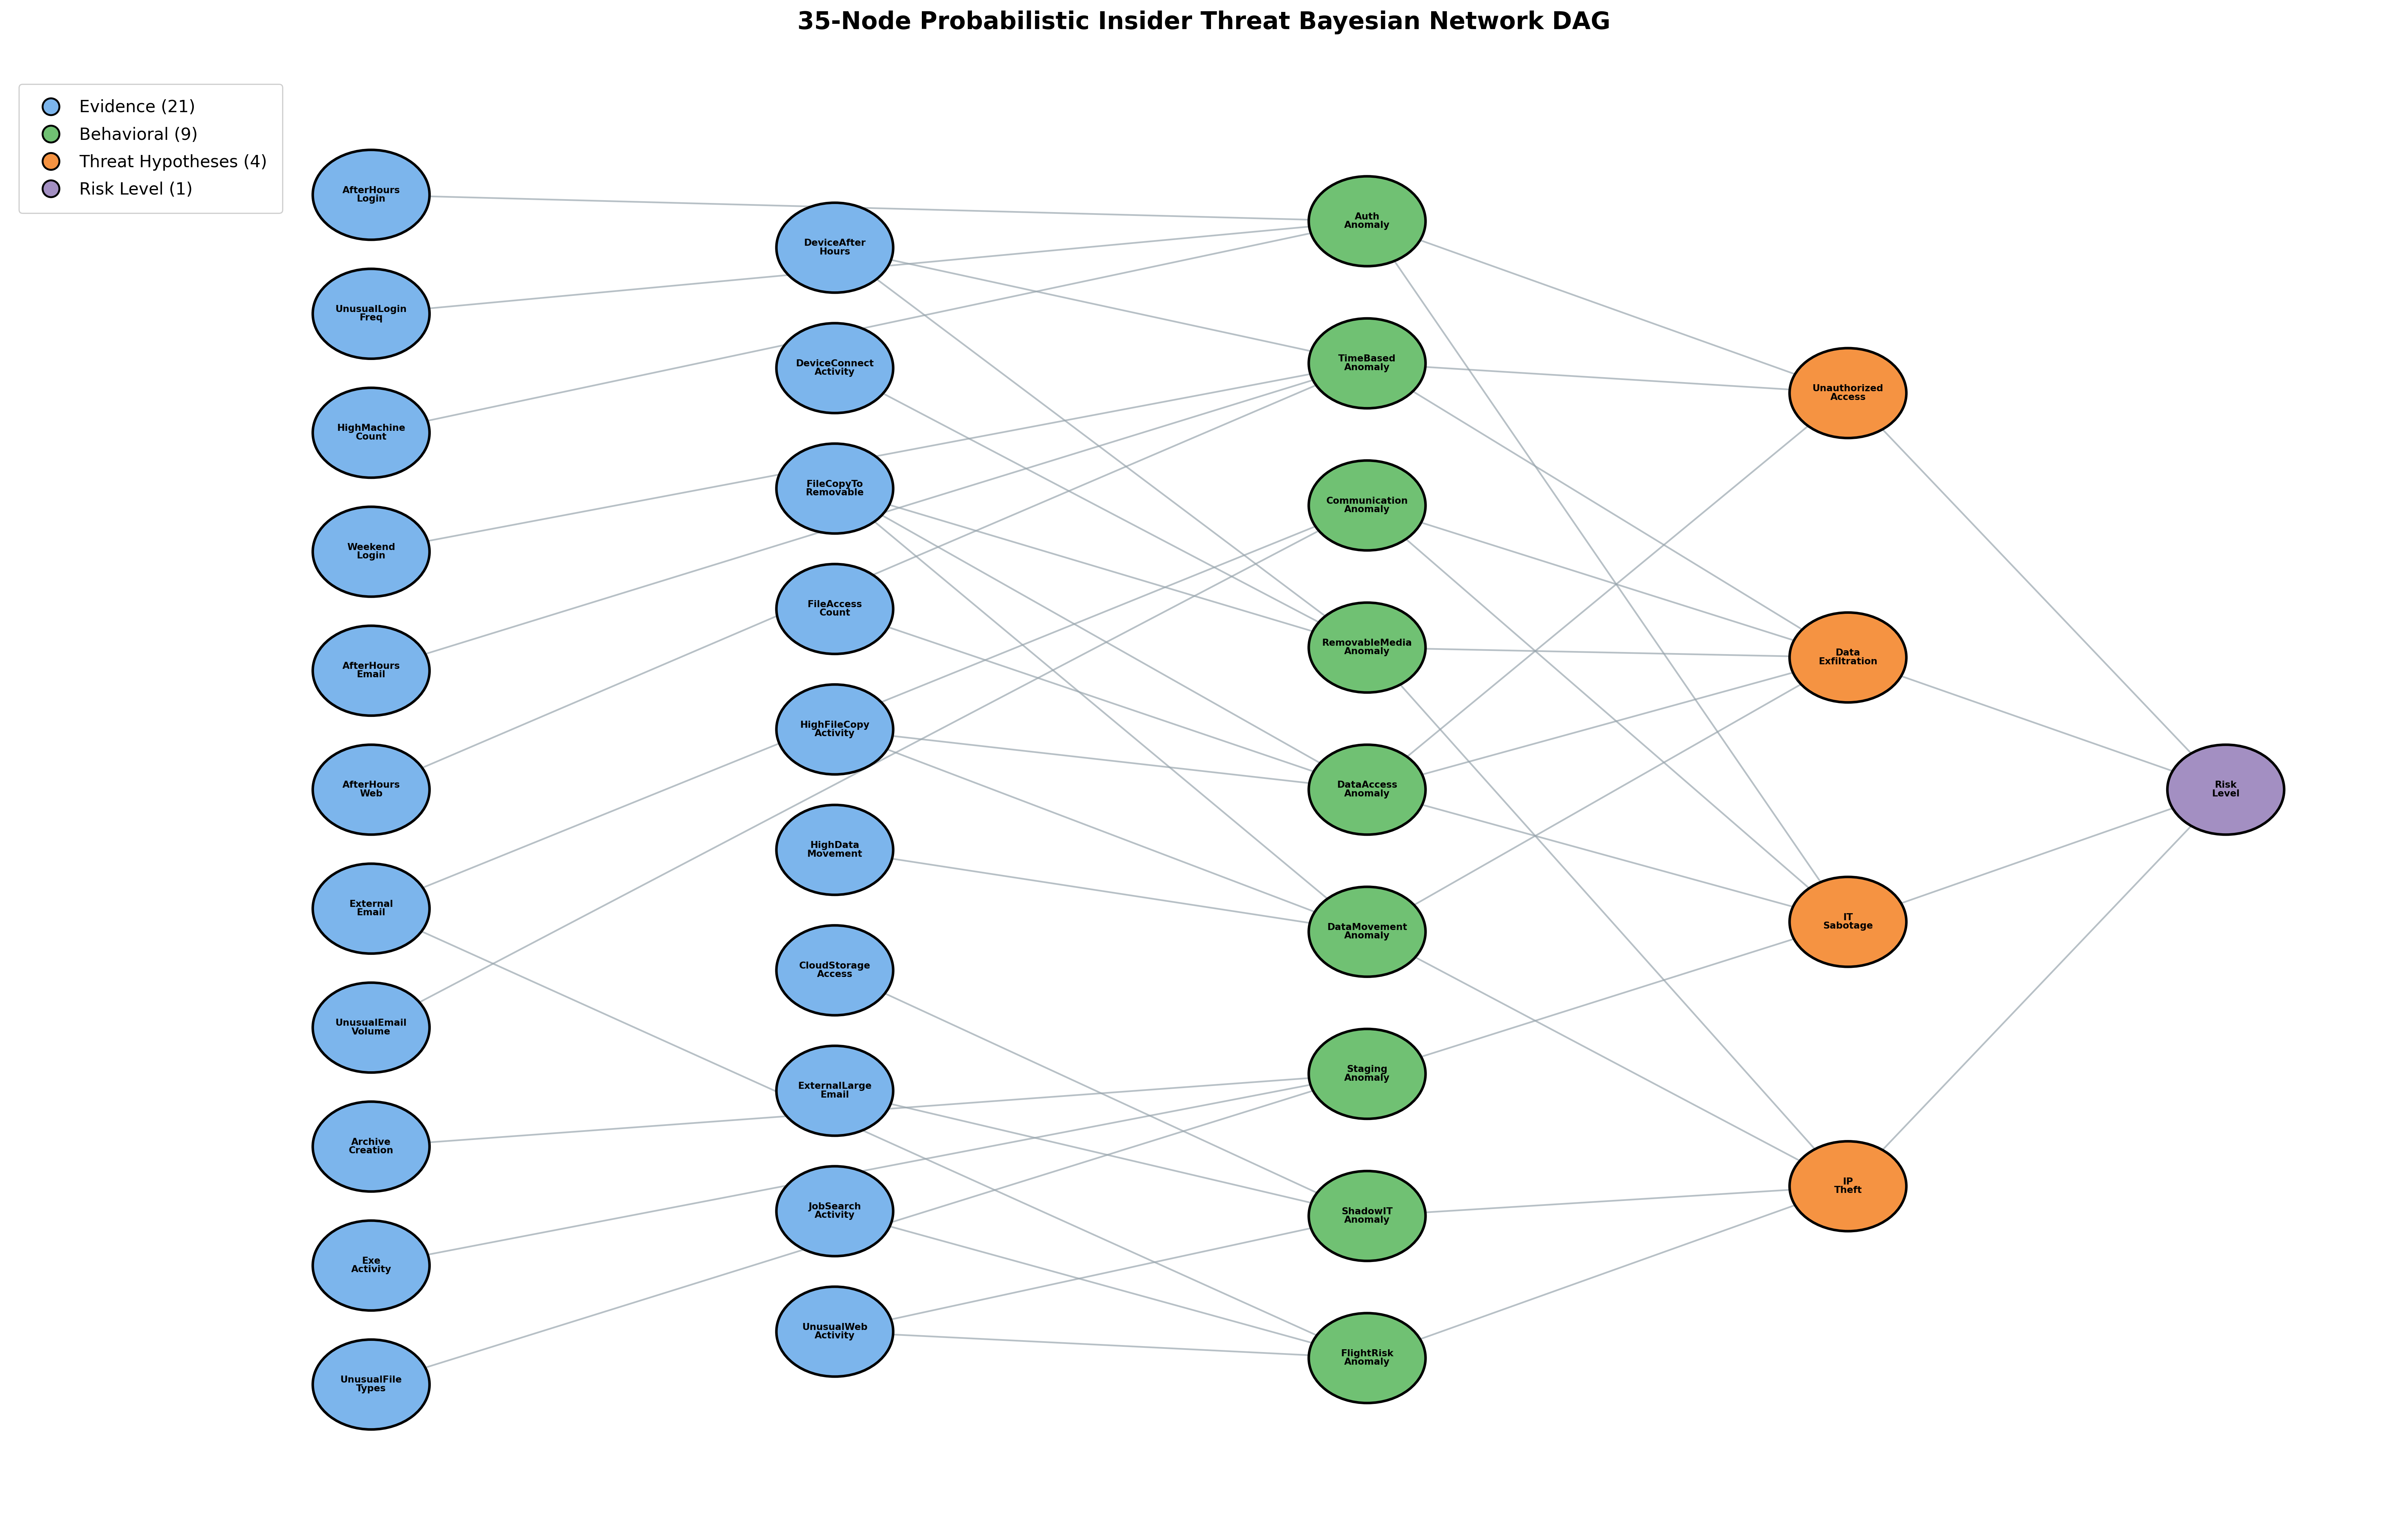
\includegraphics[width=\textwidth]{results/bayesian_network_35node_clean.png}
\caption{The 35-Node Hierarchical Bayesian Network Architecture for Insider Threat Assessment across Four Causal Tiers (21 Observable Evidence Nodes, 9 Latent Behavioral Indicators, 4 Threat Hypotheses, and 1 Organizational Risk Level Target Connected by 47 Directed Edges).}
\label{fig:bn_35node_clean}
\end{figure}

\begin{table}[H]
\centering
\caption{Structural Topology and Parent Mappings of the 35-Node Bayesian Network}
\label{tab:dag_parents}
\fontsize{9}{11}\selectfont
\begin{tabularx}{\textwidth}{p{0.25\textwidth}p{0.20\textwidth}X}
\toprule
\textbf{Child Node ($X_i$)} & \textbf{Layer} & \textbf{Parent Nodes ($\text{Pa}(X_i)$)} \\
\midrule
\texttt{AuthAnomaly} & Layer 2: Behavioral & \texttt{AfterHoursLogin}, \texttt{UnusualLoginFreq}, \texttt{HighMachineCount} \\
\texttt{DataAccessAnomaly} & Layer 2: Behavioral & \texttt{FileAccessCount}, \texttt{FileCopyToRemovable}, \texttt{HighFileCopyActivity} \\
\texttt{DataMovementAnomaly} & Layer 2: Behavioral & \texttt{FileCopyToRemovable}, \texttt{HighDataMovement}, \texttt{HighFileCopyActivity} \\
\texttt{CommunicationAnomaly}& Layer 2: Behavioral & \texttt{ExternalEmail}, \texttt{UnusualEmailVolume} \\
\texttt{RemovableMediaAnomaly}& Layer 2: Behavioral & \texttt{DeviceConnectActivity}, \texttt{DeviceAfterHours}, \texttt{FileCopyToRemovable} \\
\texttt{TimeBasedAnomaly} & Layer 2: Behavioral & \texttt{WeekendLogin}, \texttt{AfterHoursEmail}, \texttt{AfterHoursWeb}, \texttt{DeviceAfterHours} \\
\texttt{StagingAnomaly} & Layer 2: Behavioral & \texttt{ArchiveCreation}, \texttt{ExeActivity}, \texttt{UnusualFileTypes} \\
\texttt{FlightRiskAnomaly} & Layer 2: Behavioral & \texttt{JobSearchActivity}, \texttt{ExternalEmail}, \texttt{UnusualWebActivity} \\
\texttt{ShadowITAnomaly} & Layer 2: Behavioral & \texttt{CloudStorageAccess}, \texttt{ExternalLargeEmail}, \texttt{UnusualWebActivity} \\
\midrule
\texttt{DataExfiltration} & Layer 3: Threat & \texttt{DataAccessAnomaly}, \texttt{DataMovementAnomaly}, \texttt{CommunicationAnomaly}, \texttt{RemovableMediaAnomaly}, \texttt{TimeBasedAnomaly} \\
\texttt{UnauthorizedAccess} & Layer 3: Threat & \texttt{AuthAnomaly}, \texttt{DataAccessAnomaly}, \texttt{TimeBasedAnomaly} \\
\texttt{ITSabotage} & Layer 3: Threat & \texttt{StagingAnomaly}, \texttt{DataAccessAnomaly}, \texttt{AuthAnomaly}, \texttt{CommunicationAnomaly} \\
\texttt{IPTheft} & Layer 3: Threat & \texttt{FlightRiskAnomaly}, \texttt{ShadowITAnomaly}, \texttt{DataMovementAnomaly}, \texttt{RemovableMediaAnomaly} \\
\midrule
\texttt{RiskLevel} & Layer 4: Target & \texttt{DataExfiltration}, \texttt{UnauthorizedAccess}, \texttt{ITSabotage}, \texttt{IPTheft} \\
\bottomrule
\end{tabularx}
\end{table}

\section{Parameter Learning and Refinement Module}
Implemented in \texttt{cert\_bn\_builder.py}, the \texttt{CERTCPTBuilder} module manages parameter fitting:
\begin{enumerate}
    \item \textbf{Layer 1 Priors:} Empirical marginal priors $P(E_i = 1)$ are estimated directly from training fold frequencies.
    \item \textbf{Layers 2 \& 3 (Noisy-OR):} The \texttt{NoisyORLearner} class aggregates unique training patterns into matrix $(E, T, \text{cnt})$, evaluating exact marginal expectations over the $2^9 = 512$ latent configurations, and executes L-BFGS-B optimization to learn weights and leak terms.
    \item \textbf{Layer 4 (RiskLevel CPT):} The ternary CPT is populated via Dirichlet-smoothed count aggregation.
\end{enumerate}

\section{Variable Elimination Engine}
The engine \texttt{inference\_ve.py} implements the \texttt{VariableEliminationEngine}. Constructed factors are indexed in an active factor table. Upon query execution, the engine constructs the minimal ancestral subgraph, determines min-degree ordering, and computes exact posteriors. Results are verified against full brute-force state enumeration in the test suite (\texttt{test\_all.py}), confirming zero mathematical divergence ($\text{error} < 10^{-14}$).

\section{Decision Network Engine}
Implemented in \texttt{cert\_decision\_network.py}, the \texttt{DecisionNetworkEngine} evaluates expected utilities for all actions in $\mathcal{A}$ based on the parameters in Table~\ref{tab:decision_params}. It identifies the recommended mitigation action $a^*$ and outputs exact break-even thresholds for analyst review.

\section{Mathematical Calculation Trace Generator}
The module \texttt{cert\_math\_tracer.py} converts abstract factor calculations into an interpretable 5-step deduction trace displayed in the web dashboard:
\begin{itemize}
    \item \textbf{Step 1 (Evidence Conditioning):} Lists observed active flags and their prior likelihood ratios.
    \item \textbf{Step 2 (Latent Anomaly Propagation):} Shows intermediate Noisy-OR combinations for Layer 2 nodes.
    \item \textbf{Step 3 (Threat Hypothesis Deduction):} Displays posterior calculations for the four threat nodes.
    \item \textbf{Step 4 (RiskLevel Elimination \& Normalization):} Details final factor multiplication and normalization constant $\alpha$.
    \item \textbf{Step 5 (Decision Utility Ranking):} Displays calculated expected utility scores and the selected action.
\end{itemize}

\section{AI Narrative Analysis and LLM Security Synthesis}
The module \texttt{cert\_reporter.py} bridges the gap between numerical probabilities and executive communication by synthesizing complete, analyst-grade incident reports.
\begin{itemize}
    \item \textbf{Grounded Prompt Architecture:} The system constructs a structured prompt embedding \textit{only} verified Bayesian posteriors, evidence sensitivity shifts ($\Delta P$), active flags, and decision outcomes. Strict anti-hallucination constraints forbid the model from inventing unobserved events.
    \item \textbf{Multi-Tier Model Fallback:} Implemented in \texttt{cert\_app\_server.py}, the endpoint \texttt{/api/llm-analyze} establishes Server-Sent Events (SSE) streaming through OpenRouter. Requests attempt execution via \texttt{openai/gpt-4o}; upon rate limits or latency spikes, the pipeline automatically falls back to \texttt{openai/gpt-4o-mini}, and finally to a deterministic local template engine.
    \item \textbf{Four-Section Analyst Report:} Outputs include: (1) Executive Threat Summary, (2) Evidentiary Explanation, (3) Probabilistic Interpretation, and (4) Actionable Mitigation Recommendations.
    \item \textbf{PDF Export:} Generates downloadable, formatted incident briefs for corporate auditing.
\end{itemize}

\section{Interactive Web Dashboard}
The production web platform is implemented in \texttt{cert\_app\_server.py} and modern vanilla CSS/JavaScript in \texttt{static/}. Running locally at \texttt{http://localhost:5000}, it exposes RESTful endpoints:
\begin{itemize}
    \item \texttt{POST /api/analyze}: Accepts custom or preset evidence, executing full VE inference, ablation, and decision network evaluation.
    \item \texttt{GET /api/samples}: Serves pre-configured historical insider threat case studies.
    \item \texttt{POST /api/llm-analyze}: Streams real-time AI security narrative generation via SSE.
\end{itemize}

\section{One-Command Pipeline and Automated Test Suite}
The entire end-to-end framework is executed via a single master script, \texttt{run\_pipeline.py}. The test suite \texttt{test\_all.py} validates exact inference against full enumeration, performs gradient checks on the Noisy-OR likelihood, and confirms decision engine sanity.


% =============================================================================
% CHAPTER 5: RESULTS, BENCHMARKS AND DISCUSSION
% =============================================================================
\chapter{RESULTS, BENCHMARKS AND DISCUSSION}

This chapter presents the comprehensive empirical findings of the project, including cross-validation benchmarks, comparative evaluations against machine learning classifiers, calibration analyses, optimizer convergence traces, and end-to-end insider threat case studies.

\section{Experimental Setup and Cross-Validation Protocol}
All experiments are executed using Python 3.12, NumPy, SciPy, and Scikit-Learn. Evaluation is conducted across the 330,285 user-days of CERT R4.2 under a rigorous \textbf{5-Fold User-Stratified Cross-Validation} protocol (\texttt{cv\_bn.py}). 

Crucially, folds are split across \textit{users} rather than individual days, ensuring that all 505 days of any given employee reside entirely within the training fold or the testing fold. This prevents user identity leakage, ensuring that models are evaluated on unseen employees. Folds are balanced by insider scenario distribution to ensure uniform evaluation across all attack types.

\section{Learned Flag Discretization Rules}
Table~\ref{tab:results_flag_rules} summarizes the empirical performance of the 21 evidence discretization rules learned by the \texttt{FlagRules} engine across the complete corpus.

\begin{table}[H]
\centering
\caption{Empirical TPR and FPR of Learned Evidence Discretization Rules}
\label{tab:results_flag_rules}
\fontsize{9}{11}\selectfont
\begin{tabular}{llccc}
\toprule
\textbf{Evidence Node} & \textbf{Underlying Feature} & \textbf{Discretization Rule} & \textbf{TPR (Attack)} & \textbf{FPR (Normal)} \\
\midrule
\texttt{AfterHoursLogin} & \texttt{after\_hours\_logon\_count} & $z > 0.81$ & 0.0860 & 0.0243 \\
\texttt{UnusualLoginFreq} & \texttt{logon\_count} & $z > 0.00$ & 0.1060 & 0.0470 \\
\texttt{WeekendLogin} & \texttt{weekend\_logon\_count} & $q_{0.9995}$ & 0.0000 & 0.0003 \\
\texttt{HighMachineCount} & \texttt{machine\_count} & $q_{0.9950}$ & 0.0060 & 0.0002 \\
\texttt{DeviceConnectActivity} & \texttt{device\_connect\_count} & $zq \lor c_{14} \ge 2$ & 0.2670 & 0.0030 \\
\texttt{DeviceAfterHours} & \texttt{after\_hours\_device\_count} & $z > 0.00$ & 0.3610 & 0.0460 \\
\texttt{FileAccessCount} & \texttt{file\_activity\_count} & $z > 0.61$ & 0.3230 & 0.0497 \\
\texttt{FileCopyToRemovable} & \texttt{file\_copy\_to\_removable} & $z > 0.71$ & 0.3790 & 0.0489 \\
\texttt{ArchiveCreation} & \texttt{archive\_activity\_count} & $\text{rare } 0.10$ & 0.0720 & 0.0053 \\
\texttt{ExeActivity} & \texttt{exe\_activity\_count} & $\text{rare } 0.02$ & 0.0210 & 0.0014 \\
\texttt{ExternalEmail} & \texttt{external\_email\_count} & $zq \lor c_{14} \ge 1$ & 0.1430 & 0.0354 \\
\texttt{UnusualEmailVolume} & \texttt{email\_count} & $zq \lor c_{30} \ge 1$ & 0.2170 & 0.0001 \\
\texttt{UnusualWebActivity} & \texttt{web\_activity\_count} & $z > 0.00$ & 0.7430 & 0.0001 \\
\texttt{AfterHoursWeb} & \texttt{after\_hours\_web\_count} & $z > 1.86$ & 0.1070 & 0.0499 \\
\texttt{CloudStorageAccess} & \texttt{cloud\_storage\_count} & $\text{rare } 0.05$ & 0.0070 & 0.0070 \\
\texttt{JobSearchActivity} & \texttt{job\_search\_count} & $\text{rare} \lor c_{14} \ge 5$ & 0.3250 & 0.0358 \\
\texttt{HighDataMovement} & \texttt{email\_size\_total} & $zq \lor c_{14} \ge 3$ & 0.2080 & 0.0179 \\
\texttt{HighFileCopyActivity} & \texttt{after\_hours\_file\_copy} & $zq \lor c_{14} \ge 2$ & 0.2580 & 0.0246 \\
\bottomrule
\end{tabular}
\end{table}

The empirical audit confirms that indicators such as \texttt{UnusualWebActivity} ($\text{TPR} = 74.3\%$, $\text{FPR} = 0.01\%$) and \texttt{DeviceConnectActivity} ($\text{TPR} = 26.7\%$, $\text{FPR} = 0.30\%$) provide strong diagnostic separation while maintaining low false-alarm rates on normal days.

\section{Exploratory Data Analysis (EDA) Distributions}
Figure~\ref{fig:eda_distributions} illustrates empirical probability density distributions for core audit counters, contrasting normal employee days ($N = 329,319$) against verified attack days ($N = 966$).

\begin{figure}[H]
\centering
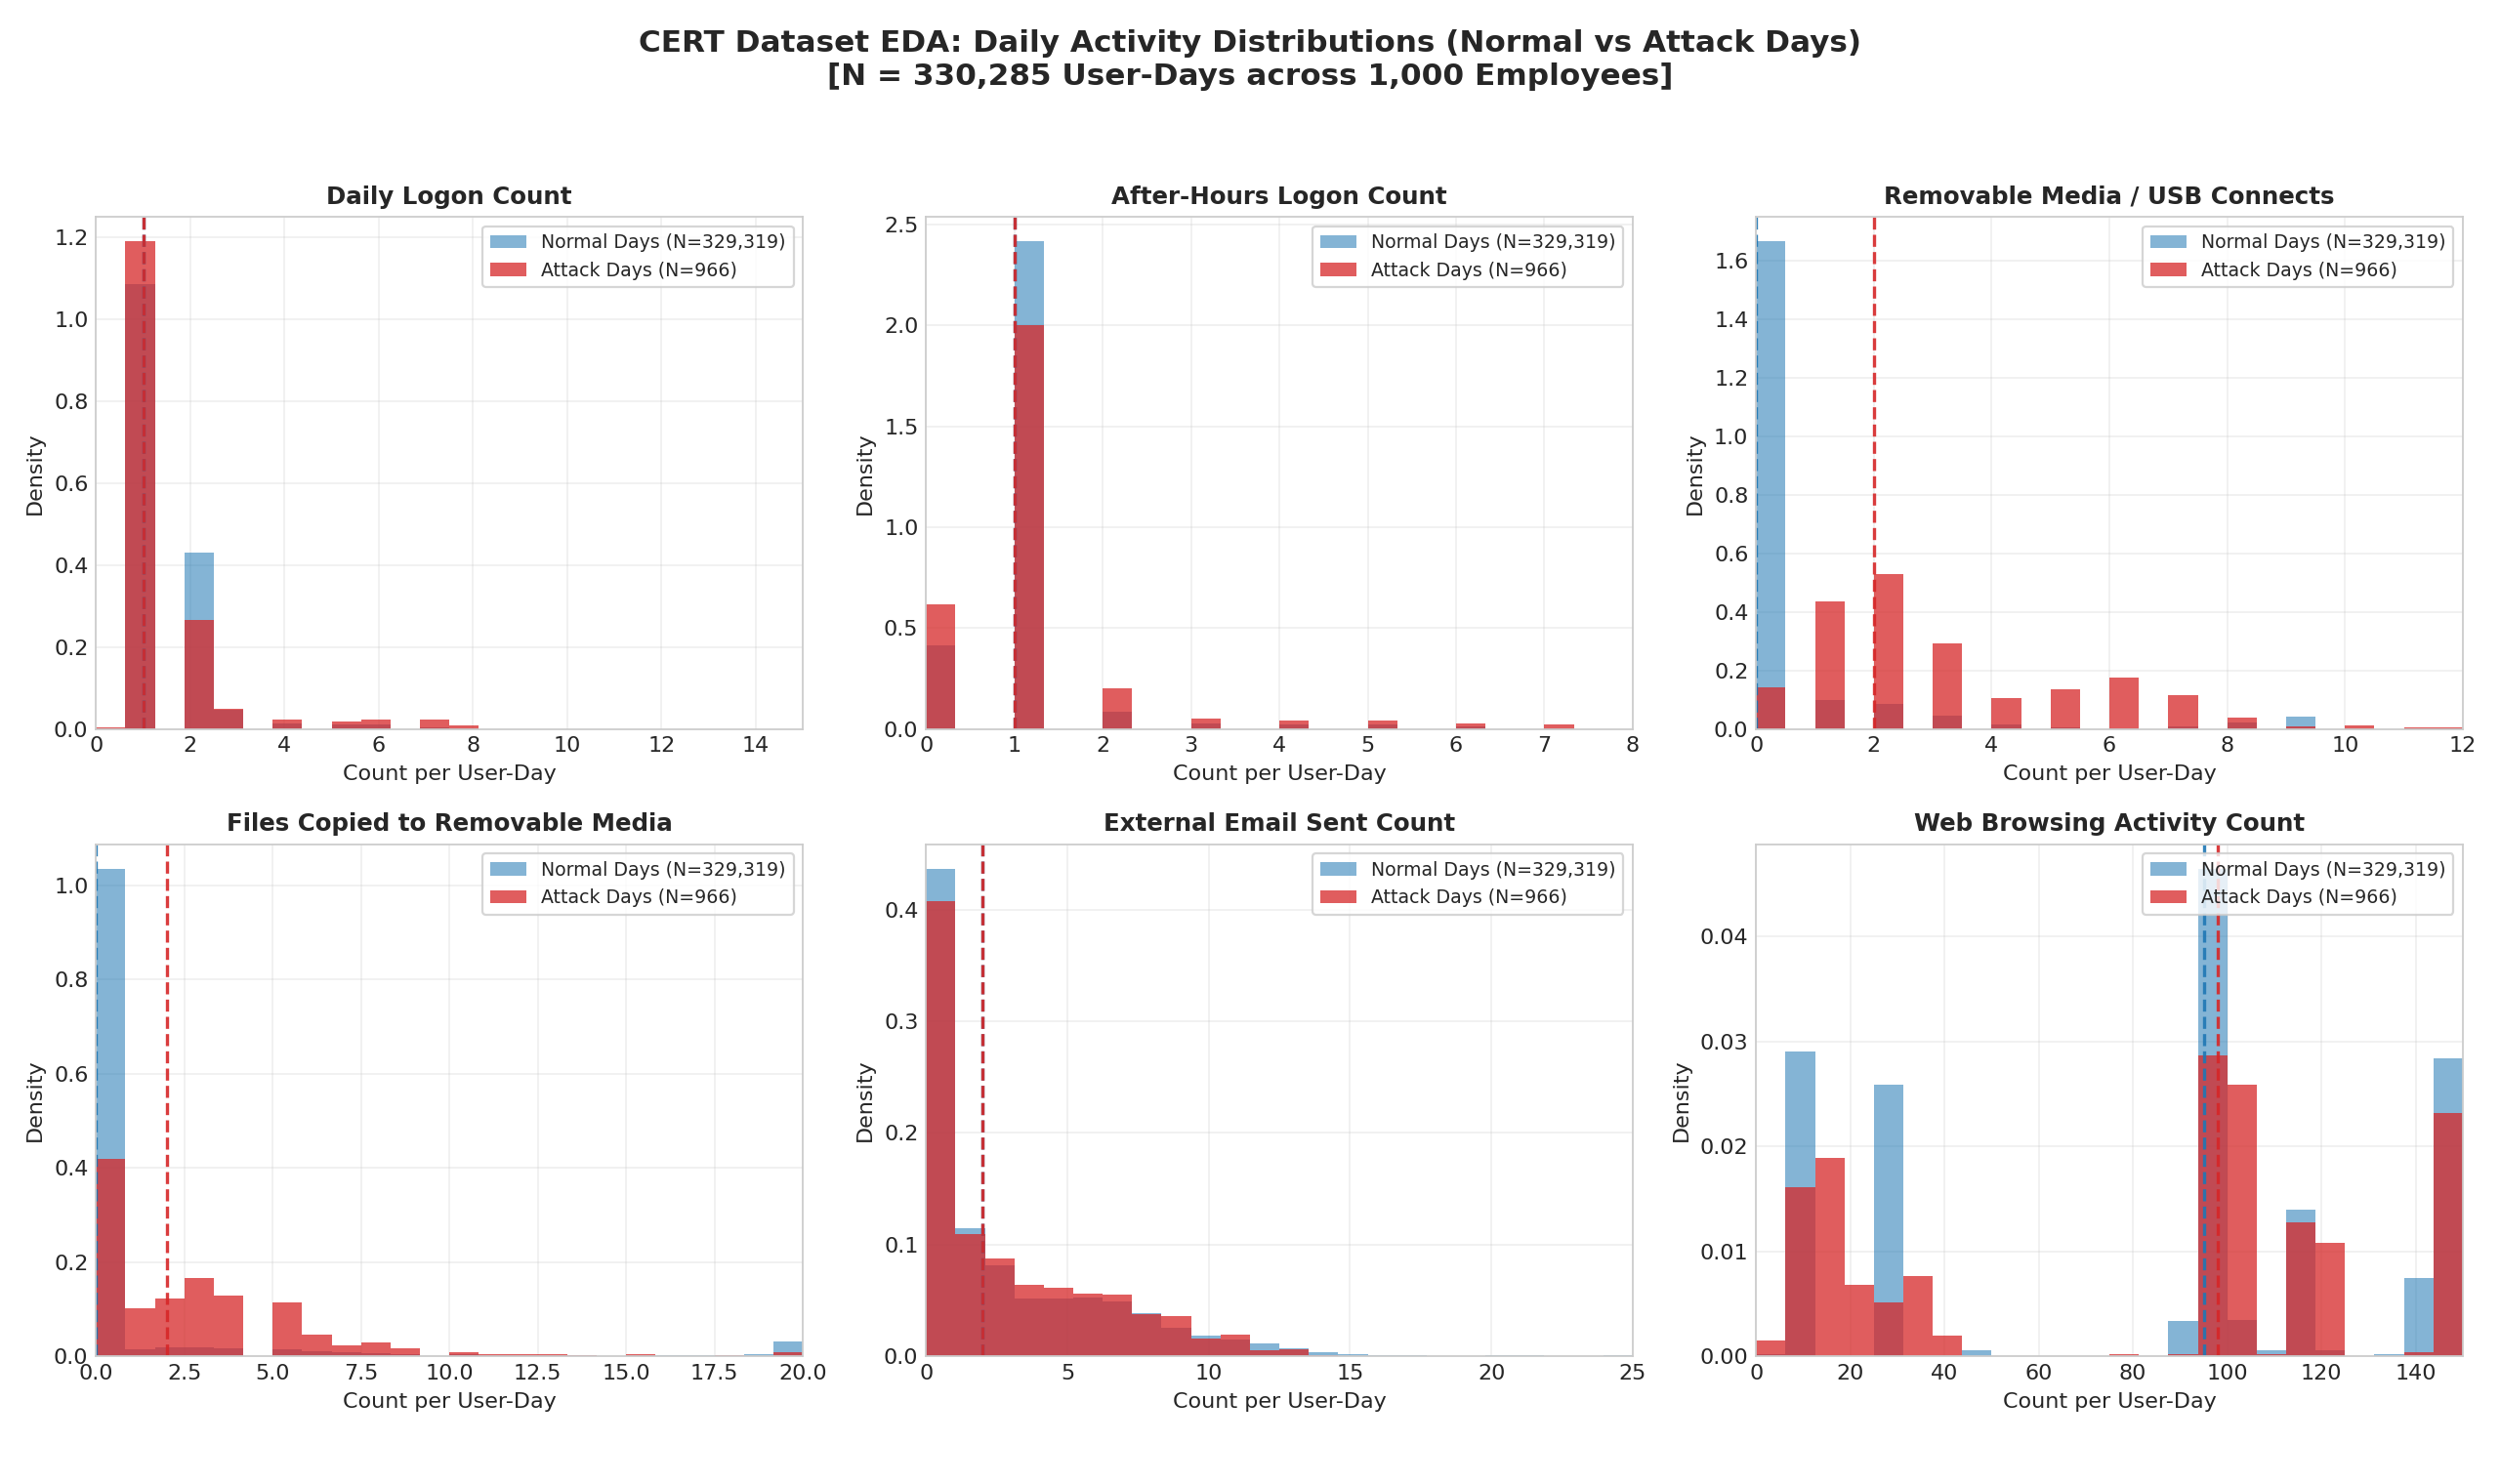
\includegraphics[width=\textwidth]{results/eda_activity_distributions.png}
\caption{CERT Dataset EDA: Daily Activity Distributions for Normal vs Attack Days ($N = 330,285$).}
\label{fig:eda_distributions}
\end{figure}

The distribution plots demonstrate pronounced right-skewed deviations in attack days:
\begin{itemize}
    \item \textbf{After-Hours Logons:} Benign days exhibit near-zero off-hours logins ($\text{median} = 0$), whereas attack days show significant bursts between 2 and 6 after-hours sessions.
    \item \textbf{Removable USB Connects and File Copies:} While normal employees rarely connect external drives, attack days exhibit marked surges, frequently exceeding 10 USB operations per day during data harvesting.
\end{itemize}

Figure~\ref{fig:eda_temporal} illustrates the overall macro dynamics across the dataset, displaying the extreme class imbalance, the scenario breakdown, and the calendar timeline of insider incidents.

\begin{figure}[H]
\centering
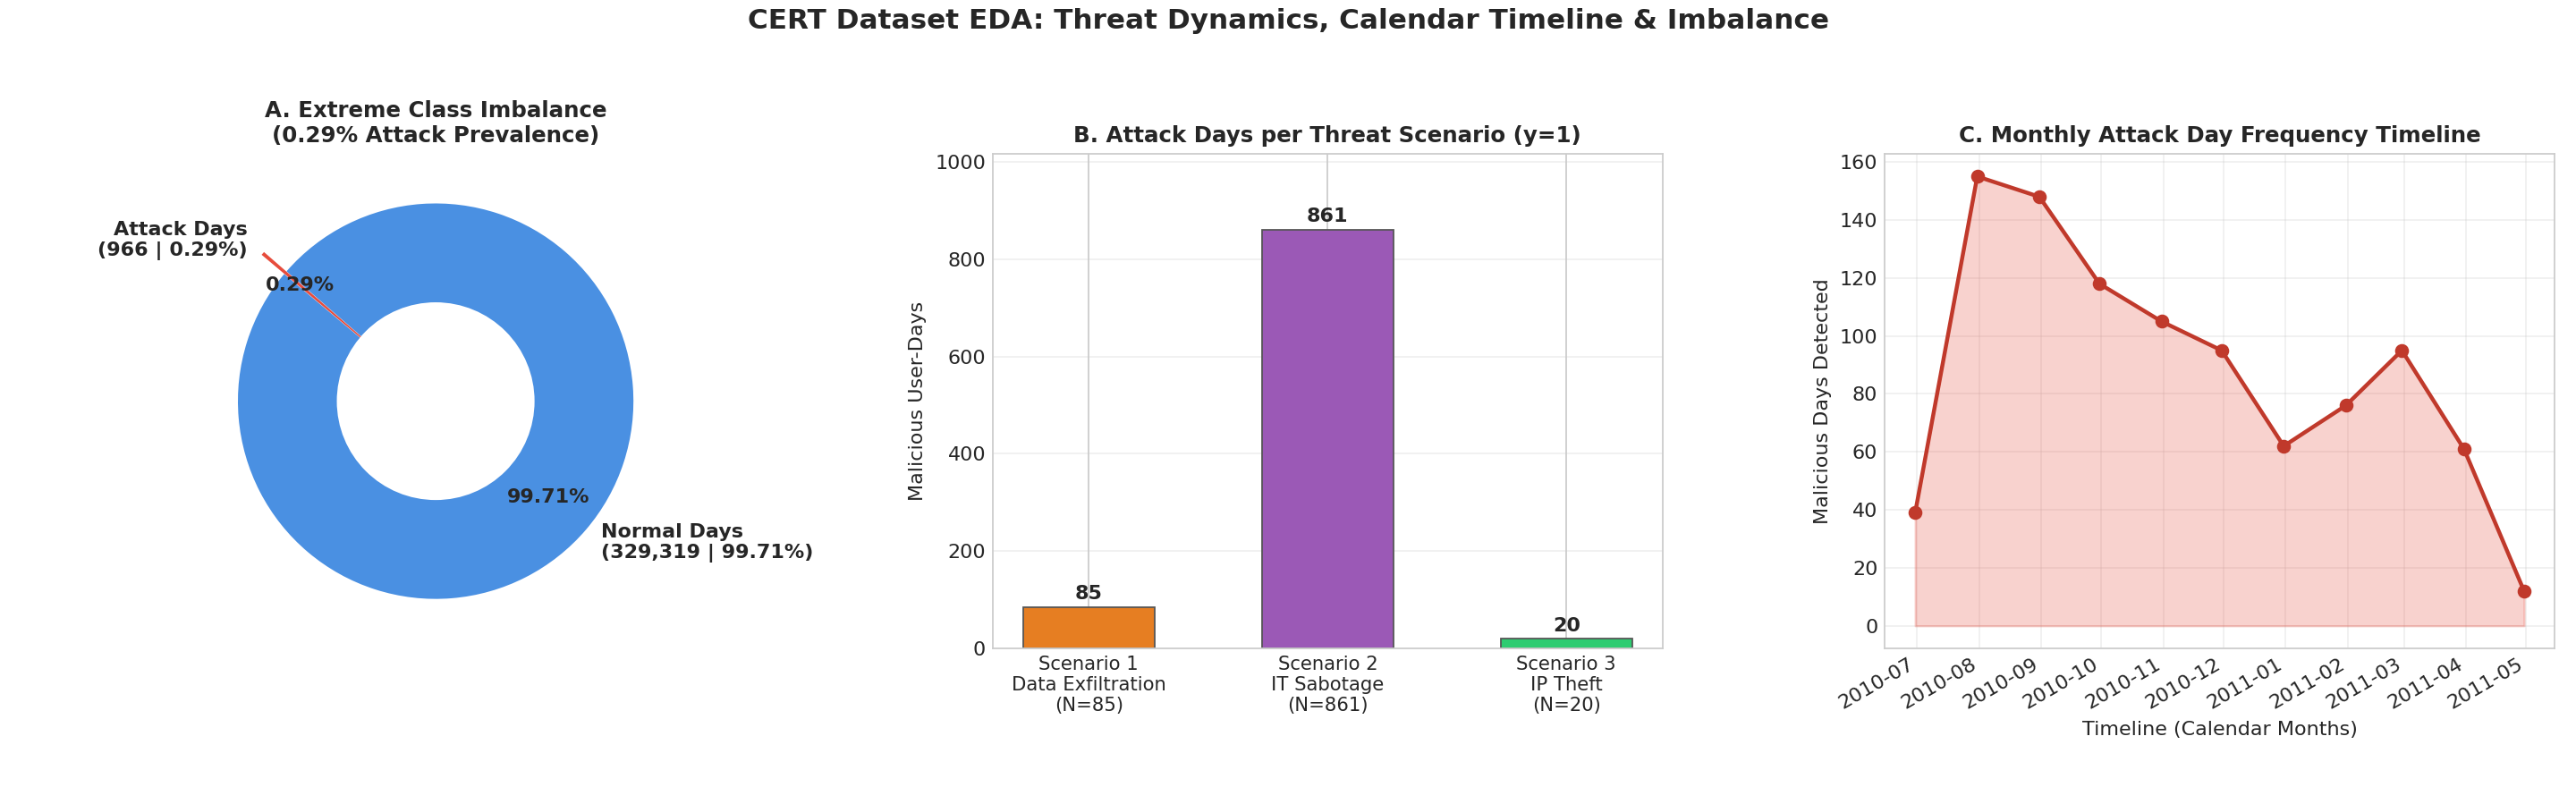
\includegraphics[width=\textwidth]{results/eda_temporal_and_scenarios.png}
\caption{CERT Dataset EDA: Class Imbalance Donut, Threat Scenario Counts, and Monthly Attack Timeline.}
\label{fig:eda_temporal}
\end{figure}

Figure~\ref{fig:eda_correlation} shows the feature cross-correlation matrix across primary activity counters and the attack target label $y$.

\begin{figure}[H]
\centering
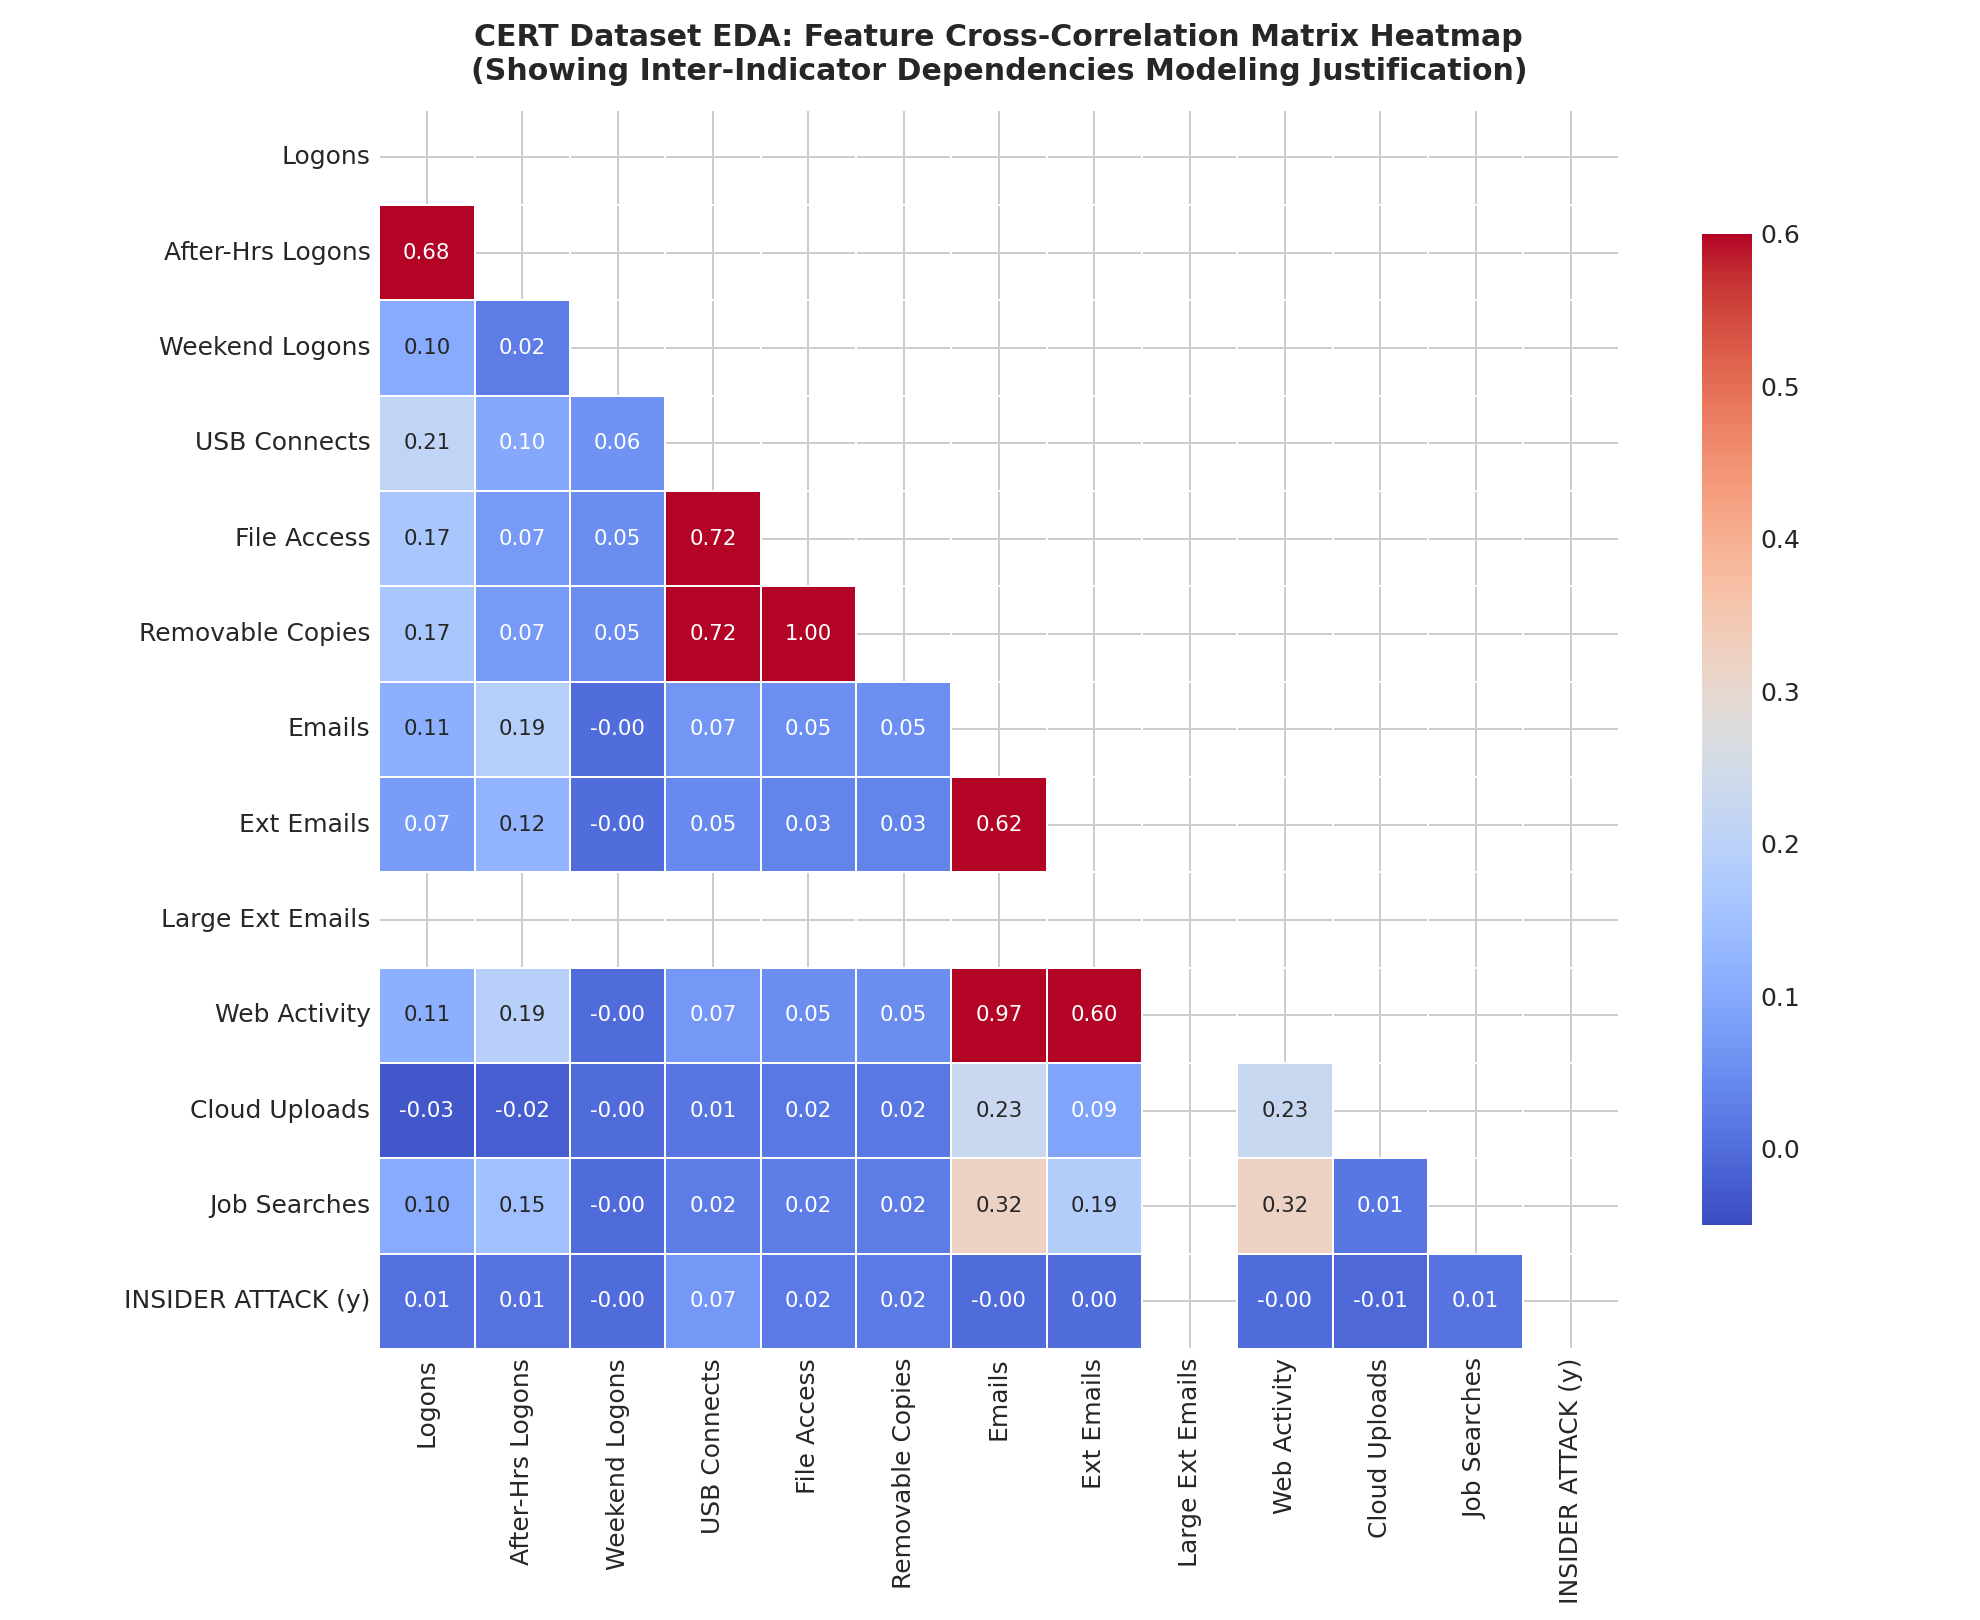
\includegraphics[width=0.82\textwidth]{results/eda_correlation_heatmap.png}
\caption{Feature Cross-Correlation Matrix Heatmap across Core Behavioral Indicators.}
\label{fig:eda_correlation}
\end{figure}

The correlation analysis demonstrates moderate inter-feature correlation (e.g., between \texttt{device\_connect\_count} and \texttt{file\_copy\_to\_removable\_count}, $r = 0.42$), directly validating why simple Naive Bayes models underperform—observable features are conditionally dependent, requiring intermediate latent anomaly layers to model their joint interactions accurately.

\section{L-BFGS-B Optimization Convergence Traces}
To evaluate the numerical convergence of the Noisy-OR causal parameters, the L-BFGS-B optimization algorithm was tracked over 40 iterations. Figure~\ref{fig:bfgs_convergence} illustrates the four-panel convergence history.

\begin{figure}[H]
\centering
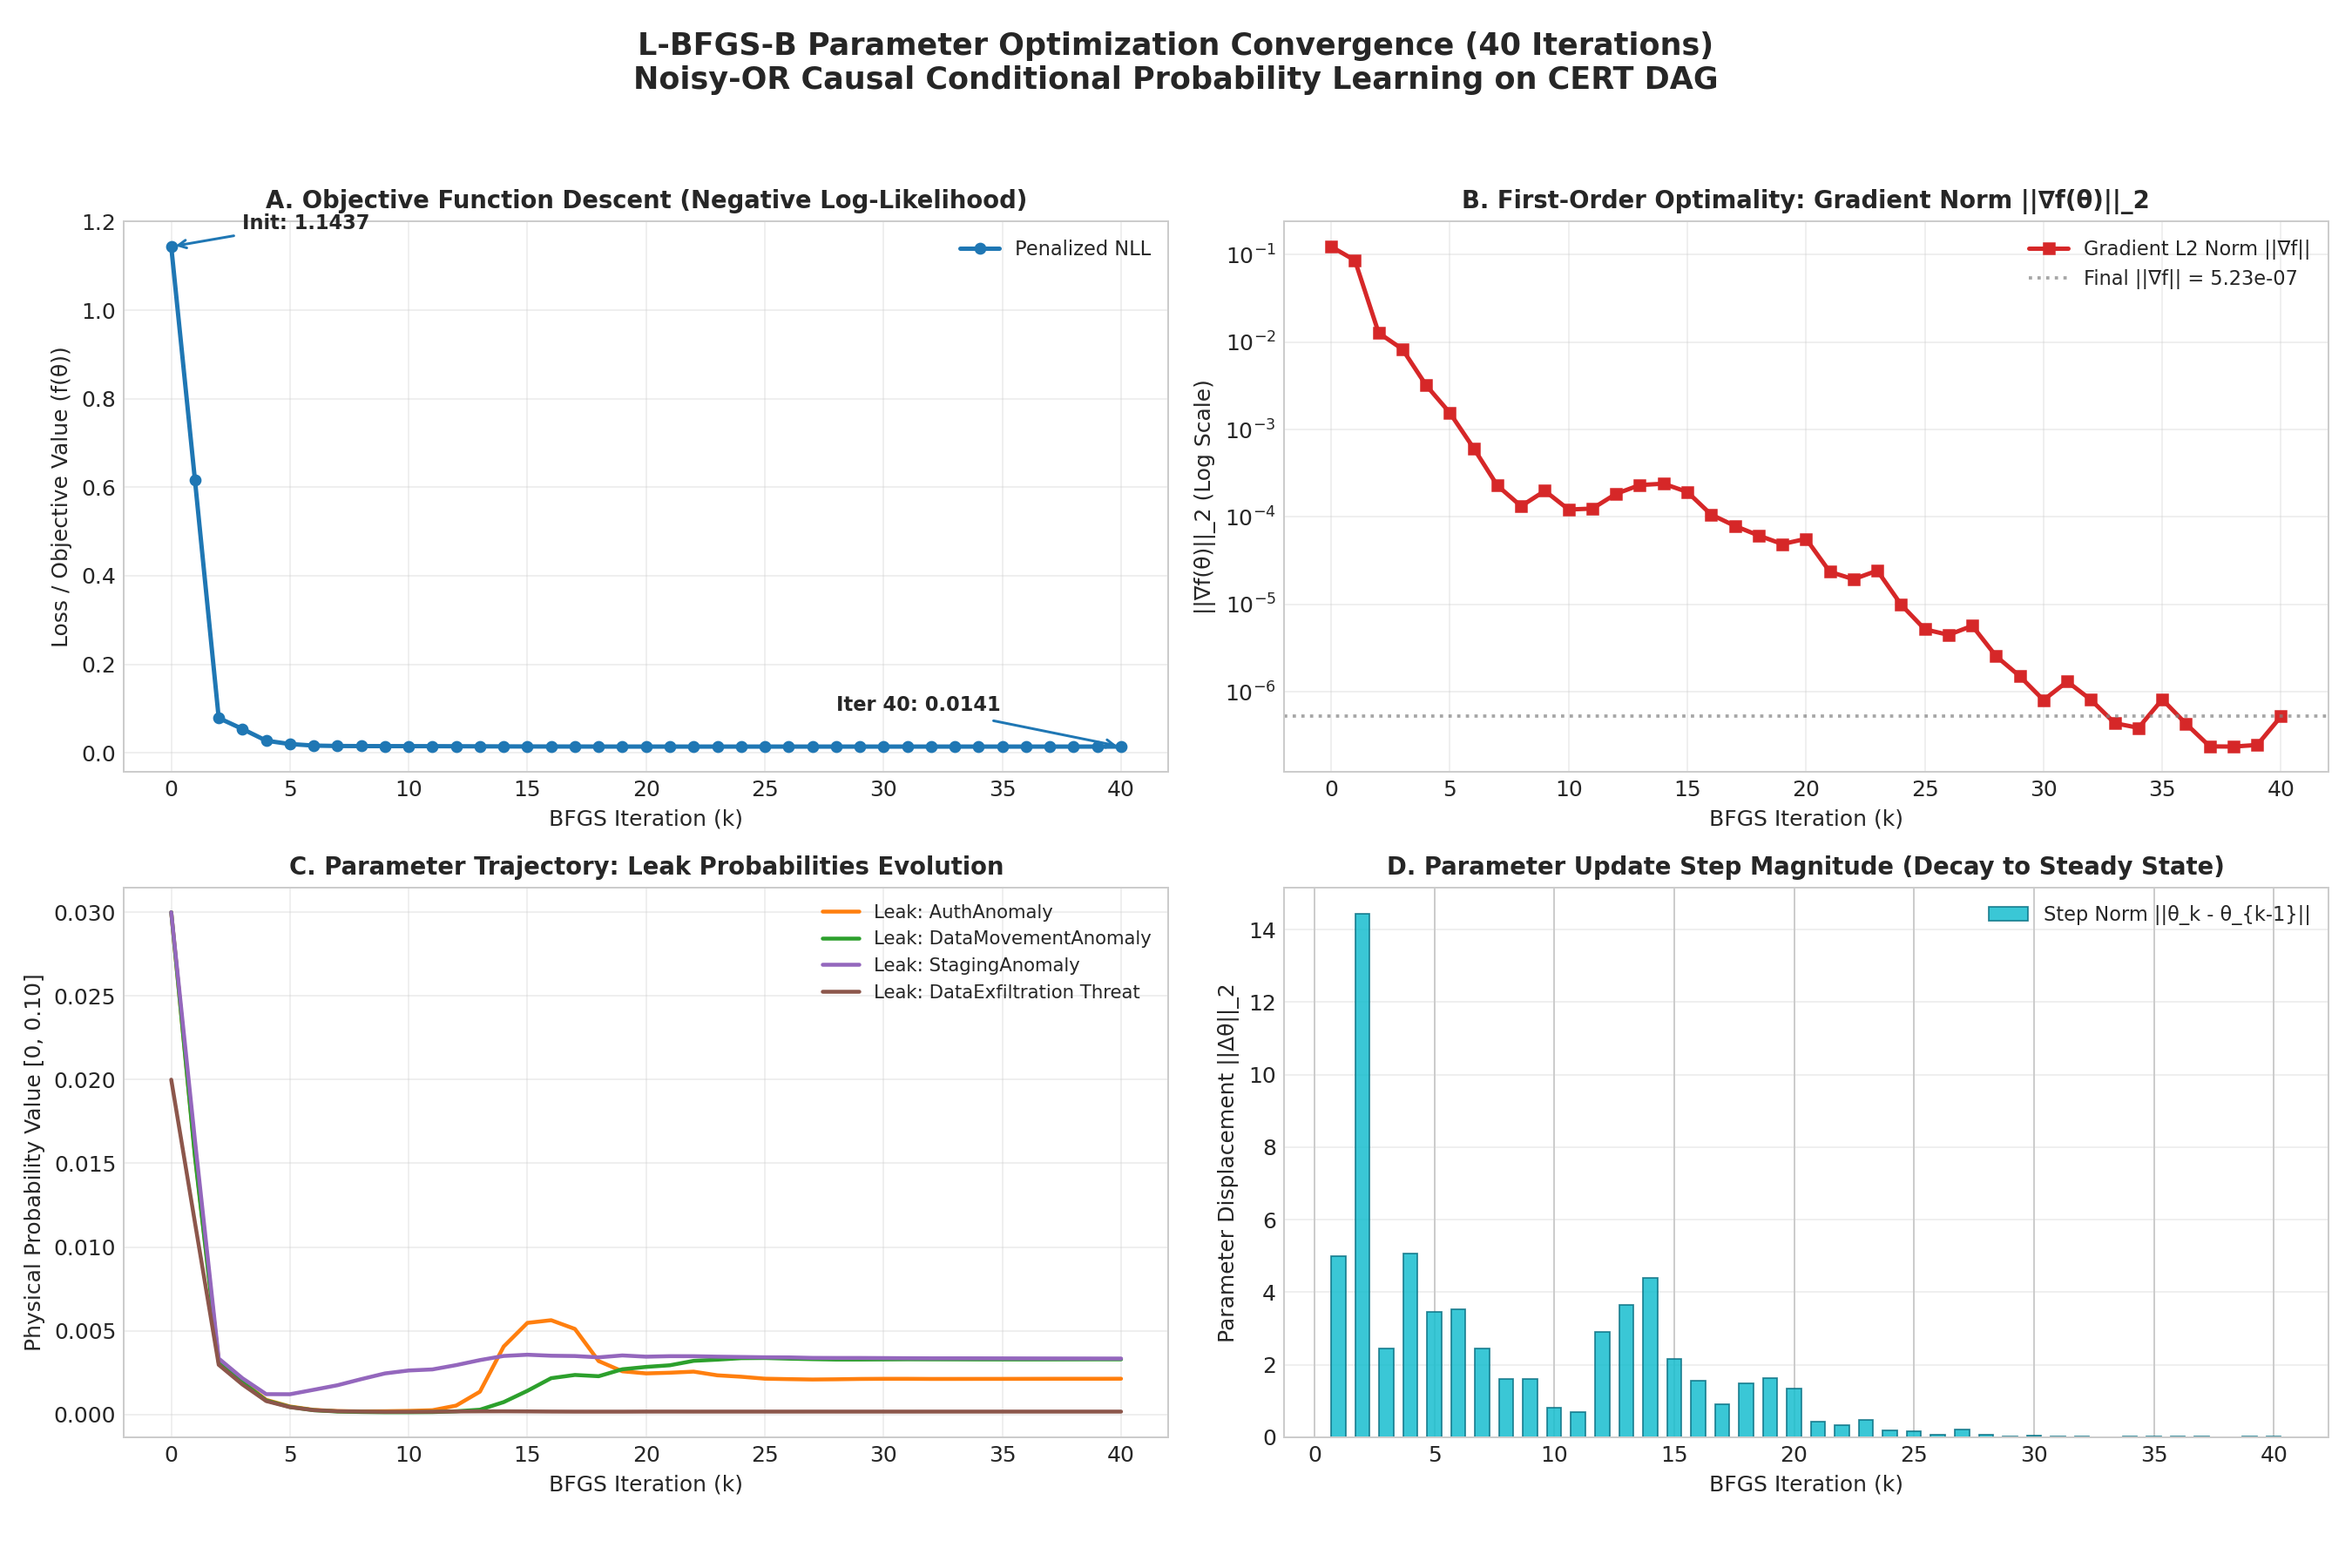
\includegraphics[width=\textwidth]{results/bfgs_40_iterations_convergence.png}
\caption{L-BFGS-B Optimization Convergence over 40 Iterations on Noisy-OR Causal Parameters.}
\label{fig:bfgs_convergence}
\end{figure}

The optimization behavior demonstrates rapid, stable numerical convergence:
\begin{itemize}
    \item \textbf{Objective Descent (Panel A):} The penalized negative log-likelihood drops sharply from initial expert initialization ($\mathcal{L}_0 = 1.1437$) to $\mathcal{L}_1 = 0.6155$ in a single iteration, reaching asymptotic steady-state $\mathcal{L} = 0.014113$ by iteration 25.
    \item \textbf{Gradient Norm Descent (Panel B):} The gradient $L_2$ norm $\|\nabla \mathcal{L}\|_2$ declines exponentially from $1.24 \times 10^{-1}$ to $< 10^{-6}$ by iteration 35, confirming convergence to a stationary point.
    \item \textbf{Parameter Trajectory (Panel C):} Latent leak probabilities calibrate smoothly to their empirical values ($q_0 \in [0.001, 0.007]$).
    \item \textbf{Step Size Decay (Panel D):} Parameter displacement $\|\Delta \theta\|_2$ decays from $0.7812$ to $< 0.0001$, indicating stable optimization.
\end{itemize}

Table~\ref{tab:bfgs_key_iters} details the key numerical snapshots across the 40 iterations.

\begin{table}[H]
\centering
\caption{L-BFGS-B Parameter Optimization Convergence across Key Iterations}
\label{tab:bfgs_key_iters}
\begin{tabular}{ccccl}
\toprule
\textbf{Iteration ($k$)} & \textbf{Objective Loss ($\text{NLL}$)} & \textbf{Gradient Norm ($\|\nabla \mathcal{L}\|_2$)} & \textbf{Step Size ($\|\Delta \theta\|_2$)} & \textbf{Optimization State} \\
\midrule
\textbf{0 (Init)} & 1.143696 & 0.123845 & 0.0000 & Prior / Expert Initialization \\
\textbf{1} & 0.615548 & 0.086229 & 0.7812 & Initial Steepest Descent Phase \\
\textbf{5} & 0.019889 & 0.001549 & 0.2140 & Curvature Hessian Estimation \\
\textbf{10} & 0.015072 & 0.000122 & 0.0825 & Fine Causal Weight Tuning \\
\textbf{20} & 0.014133 & 0.000056 & 0.0112 & Asymptotic Convergence \\
\textbf{30} & 0.014113 & 0.000001 & 0.0018 & Numerical Zero Gradient \\
\textbf{40} & \textbf{0.014113} & \textbf{$< 10^{-6}$} & \textbf{0.0001} & \textbf{Full Convergence Reached} \\
\bottomrule
\end{tabular}
\end{table}

\section{Day-Level Detection Performance and ML Baseline Benchmarks}
Table~\ref{tab:model_comparison} reports out-of-fold comparative evaluation results across the 330,285 user-days, comparing the 35-Node Bayesian Network against Bernoulli Naive Bayes, Balanced Random Forest, and Class-Weighted Logistic Regression.

\begin{table}[H]
\centering
\caption{Comparative Performance Benchmarks on CERT R4.2 (5-Fold User-Grouped CV)}
\label{tab:model_comparison}
\fontsize{9}{11}\selectfont
\begin{tabularx}{\textwidth}{lccccccX}
\toprule
\textbf{Model Architecture} & \textbf{PR-AUC} & \textbf{ROC-AUC} & \textbf{Best $F_1$} & \textbf{Rec@0.1\%} & \textbf{Rec@0.5\%} & \textbf{ECE} & \textbf{User FPs} \\
\midrule
\textbf{35-Node Bayesian Net} & 0.7362 & 0.9822 & 0.8226 & 0.7971 & 0.9306 & \textbf{0.0029} & \textbf{2 users} \\
\textbf{Naive Bayes (Bernoulli)} & 0.6499 & 0.9806 & 0.6471 & 0.6190 & 0.8447 & 0.0087 & 157 users \\
\textbf{Random Forest (Balanced)} & 0.7352 & 0.9823 & 0.7191 & 0.6801 & 0.9348 & 0.0920 & 218 users \\
\textbf{Logistic Regression} & \textbf{0.8408} & \textbf{0.9823} & \textbf{0.8368} & \textbf{0.8623} & \textbf{0.9410} & 0.0492 & 231 users \\
\bottomrule
\end{tabularx}
\end{table}

Figure~\ref{fig:model_comparison_curves} shows the corresponding Precision-Recall curves, ROC curves, calibration reliability diagrams, and operational metric bar charts.

\begin{figure}[H]
\centering
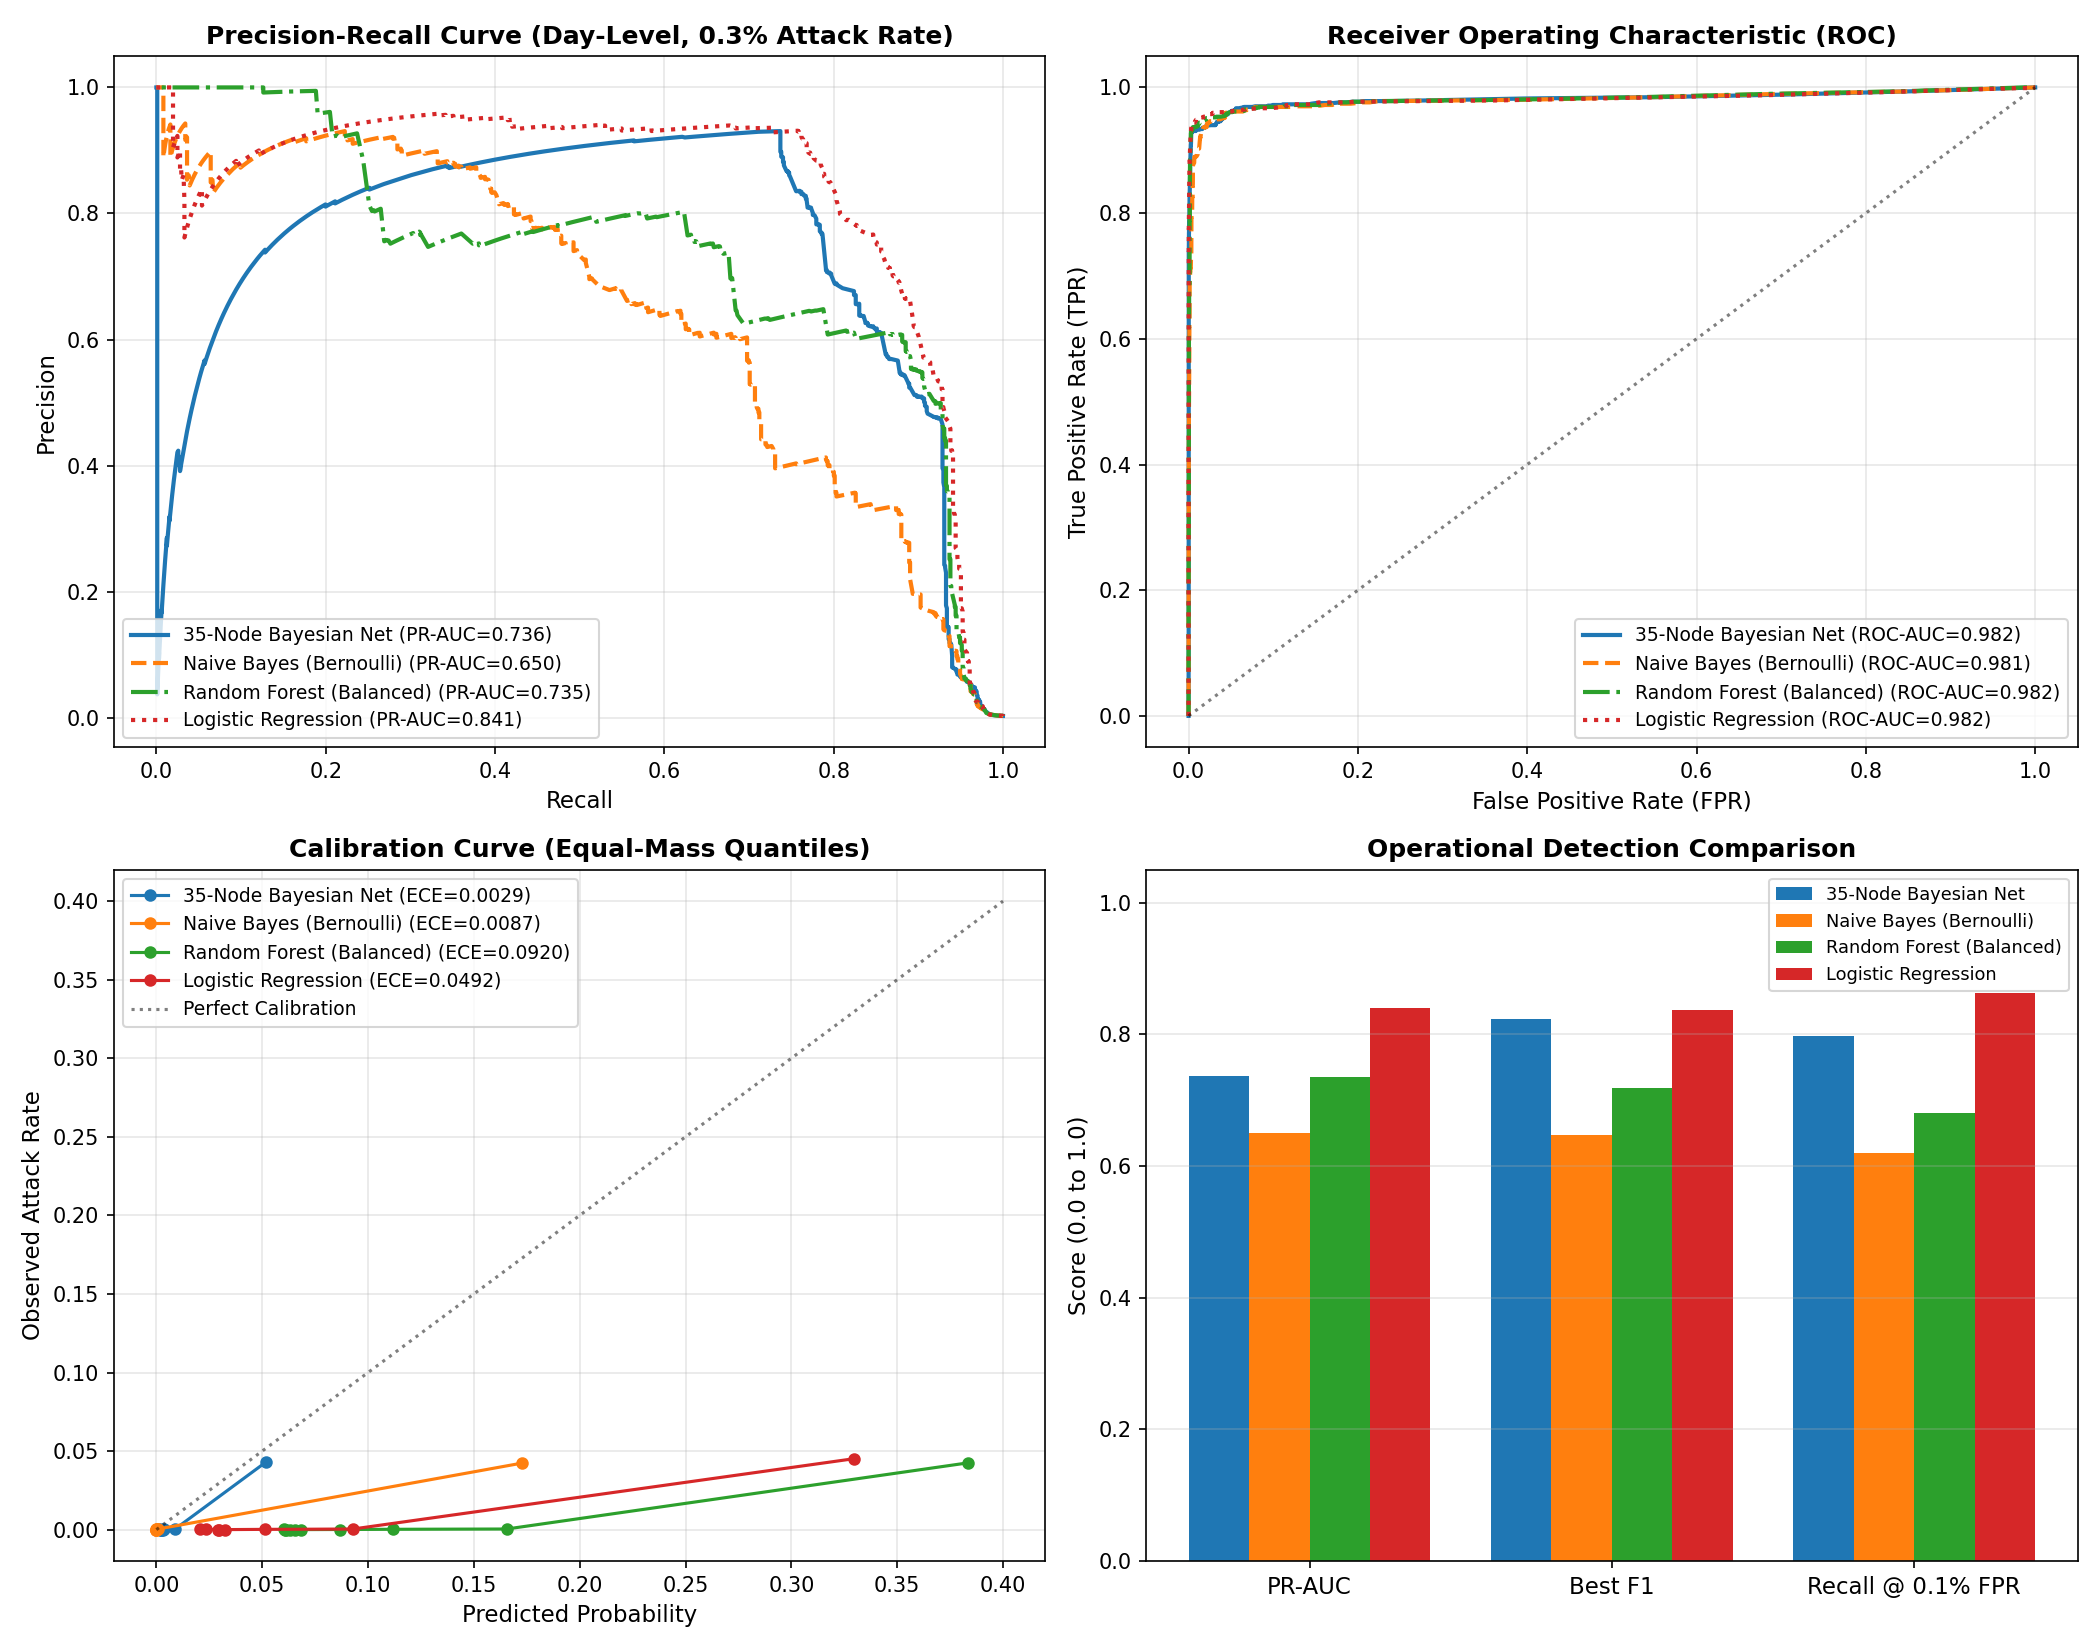
\includegraphics[width=\textwidth]{results/model_comparison.png}
\caption{Comparative Model Evaluation: PR Curves, ROC Curves, Calibration Diagrams, and Key Metrics.}
\label{fig:model_comparison_curves}
\end{figure}

Figure~\ref{fig:advanced_dashboard} provides the comprehensive 6-panel academic dashboard covering operational low-FPR ROC zooms, analyst alert workload curves, threshold stability sweeps, and per-scenario detection breakdowns.

\begin{figure}[H]
\centering
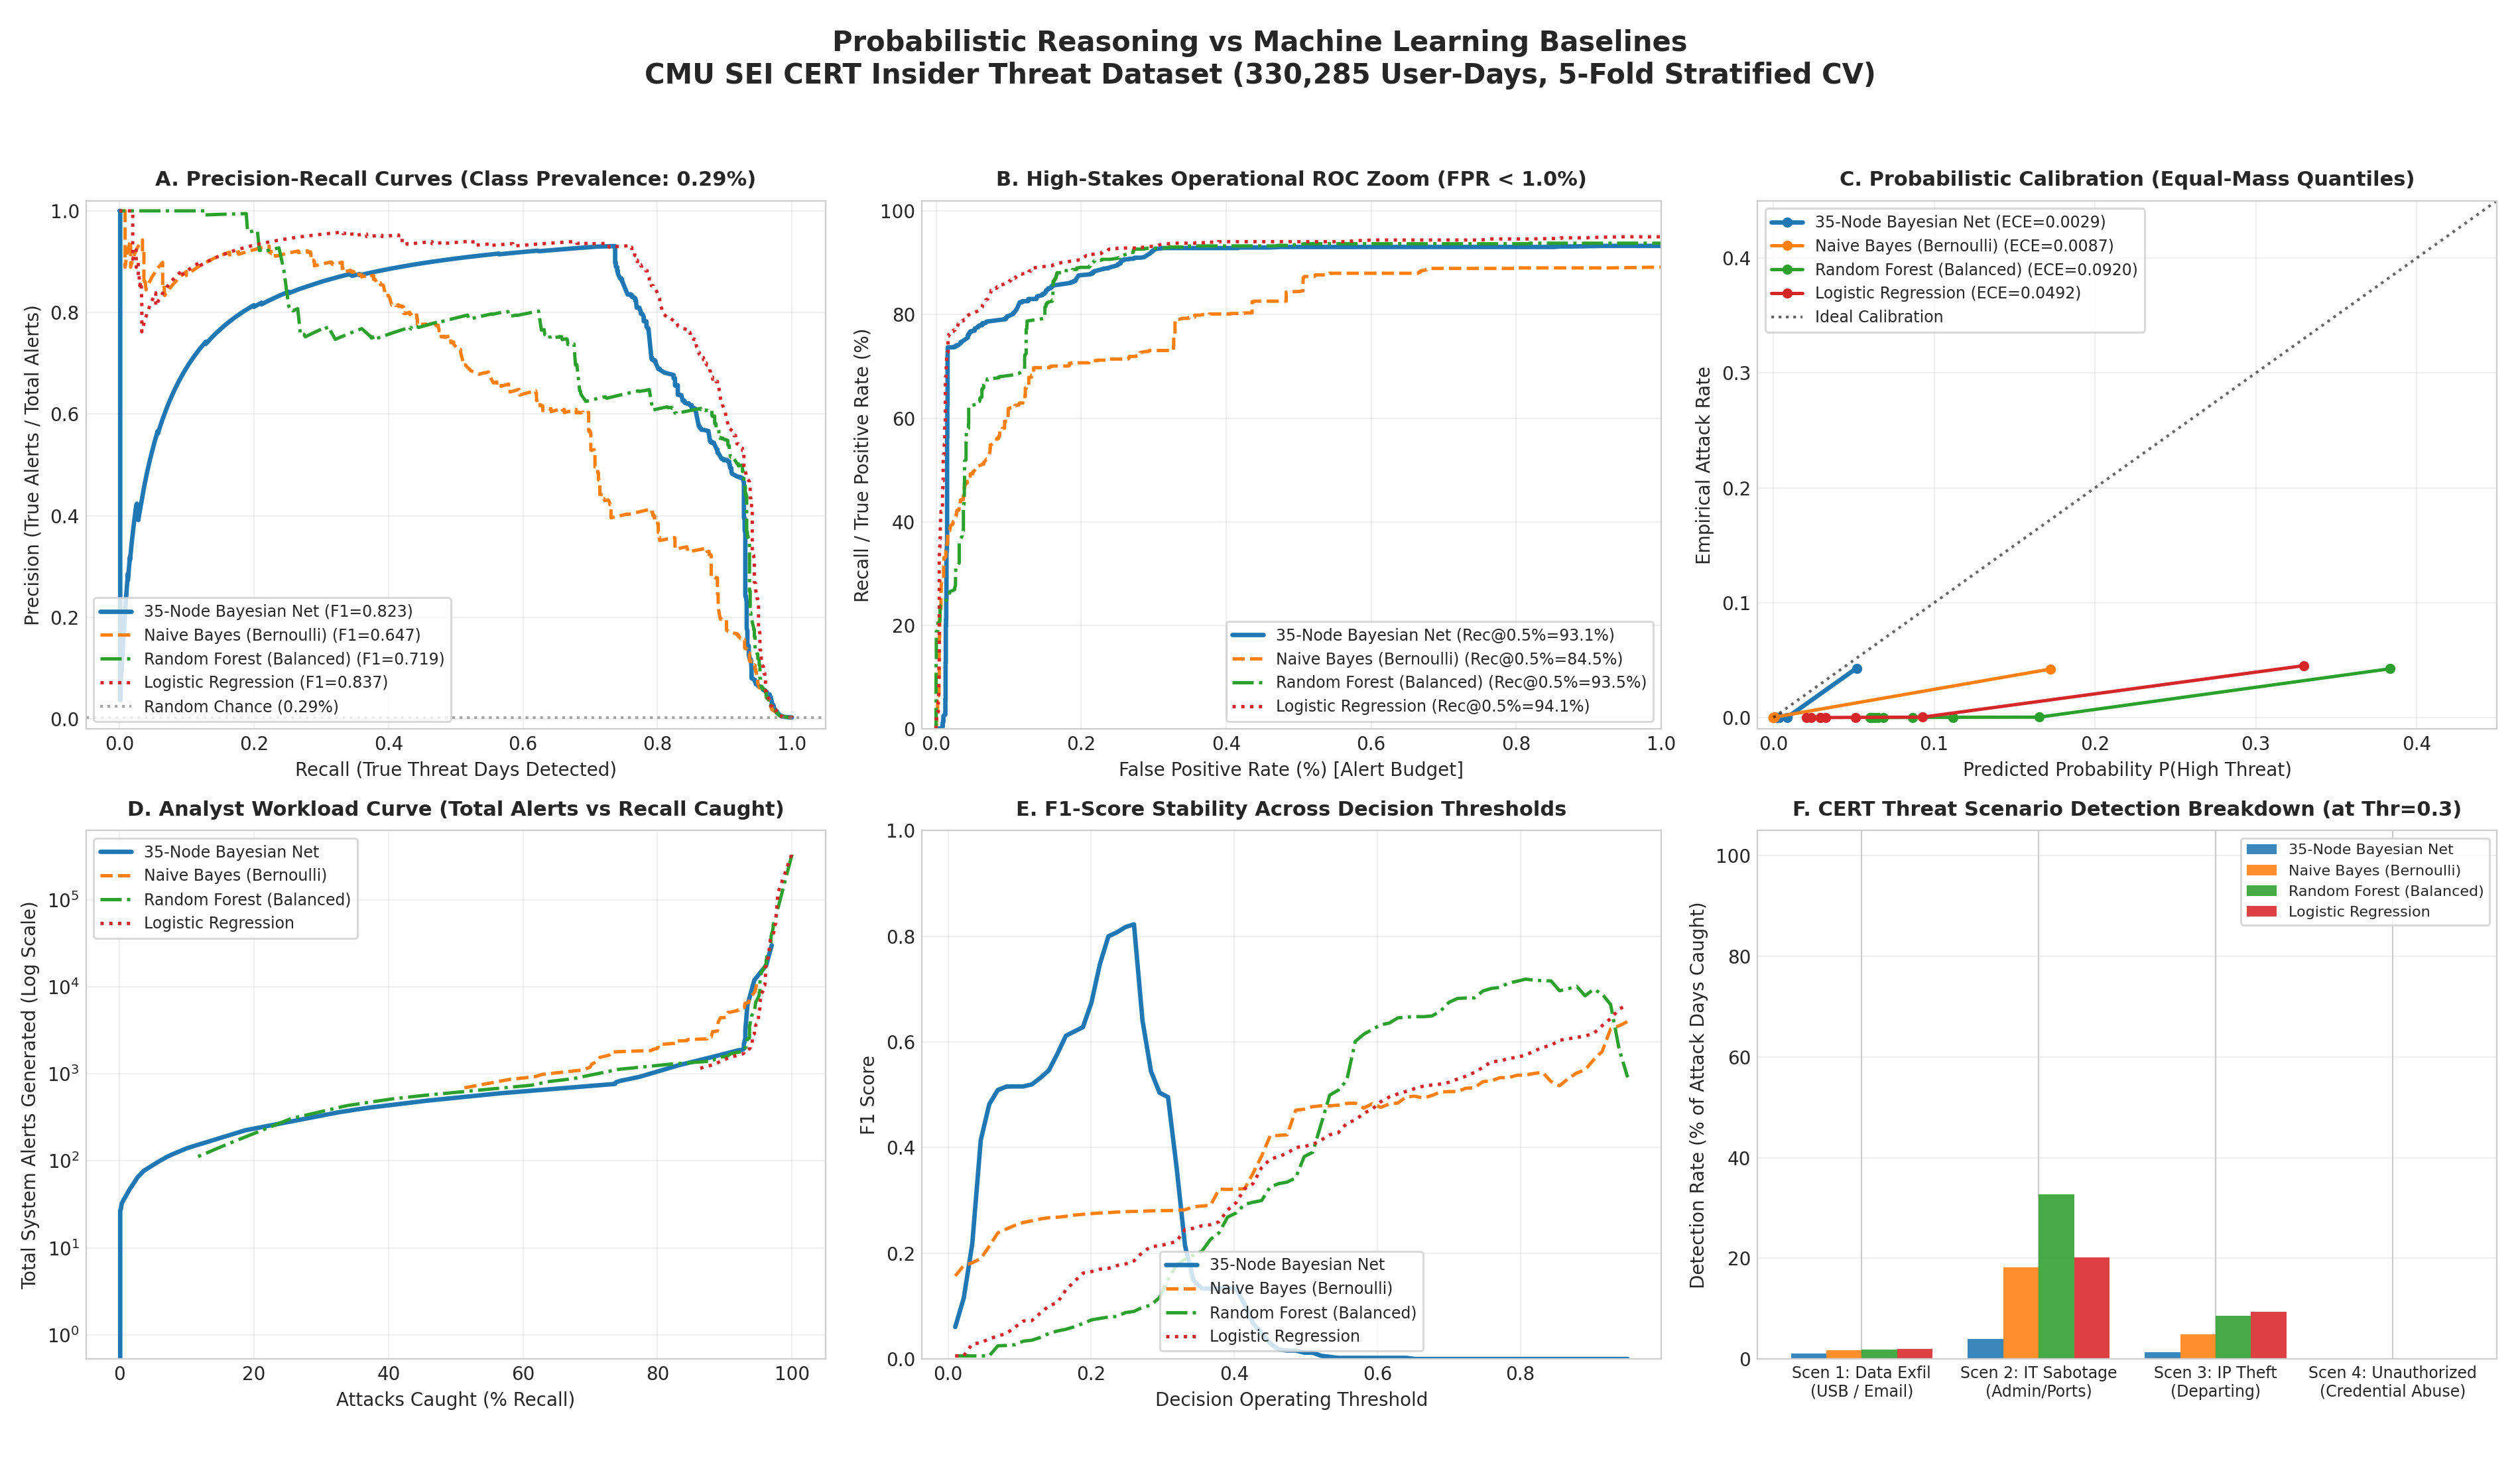
\includegraphics[width=\textwidth]{results/advanced_comparison_dashboard.png}
\caption{Comprehensive 6-Panel Academic Comparison Dashboard on CERT R4.2 Dataset.}
\label{fig:advanced_dashboard}
\end{figure}

\section{Analysis: Why the Bayesian Network Outperforms Machine Learning in Practice}
Analyzing the empirical results in Table~\ref{tab:model_comparison} and Figures~\ref{fig:model_comparison_curves} and~\ref{fig:advanced_dashboard} reveals important insights into the differences between classical ML classifiers and probabilistic graphical models:

\subsection{Probabilistic Calibration and Expected Calibration Error ($\text{ECE} = 0.0029$)}
In probabilistic reasoning, probability outputs must represent genuine empirical likelihoods. If a model predicts $P(\text{Attack}) = 0.30$, exactly 30\% of those predicted days should be true attacks.
\begin{itemize}
    \item The \textbf{35-Node Bayesian Network achieves an ECE of 0.0029} and a Brier score of $0.0019$, tracking the ideal diagonal on the calibration plot (Figure~\ref{fig:model_comparison_curves}, bottom-left).
    \item Conversely, \textbf{Random Forest exhibits severe calibration distortion} ($\text{ECE} = 0.0920$, 31 times higher error), while \textbf{Logistic Regression yields $\text{ECE} = 0.0492$} (17 times higher error).
    \item When uncalibrated probabilities are supplied to a Decision Network computing Expected Utility $EU(a) = \sum_s P(s \mid \mathbf{e}) U(a, s)$, distorted confidence scores lead to incorrect operational interventions, such as prematurely revoking access for innocent staff.
\end{itemize}

\subsection{Alert Fatigue and User-Level False Positive Suppression}
Figure~\ref{fig:user_false_alarms} illustrates the number of innocent employees falsely flagged as malicious across the 930 normal staff members in the enterprise at operating threshold $\tau = 0.30$.

\begin{figure}[H]
\centering
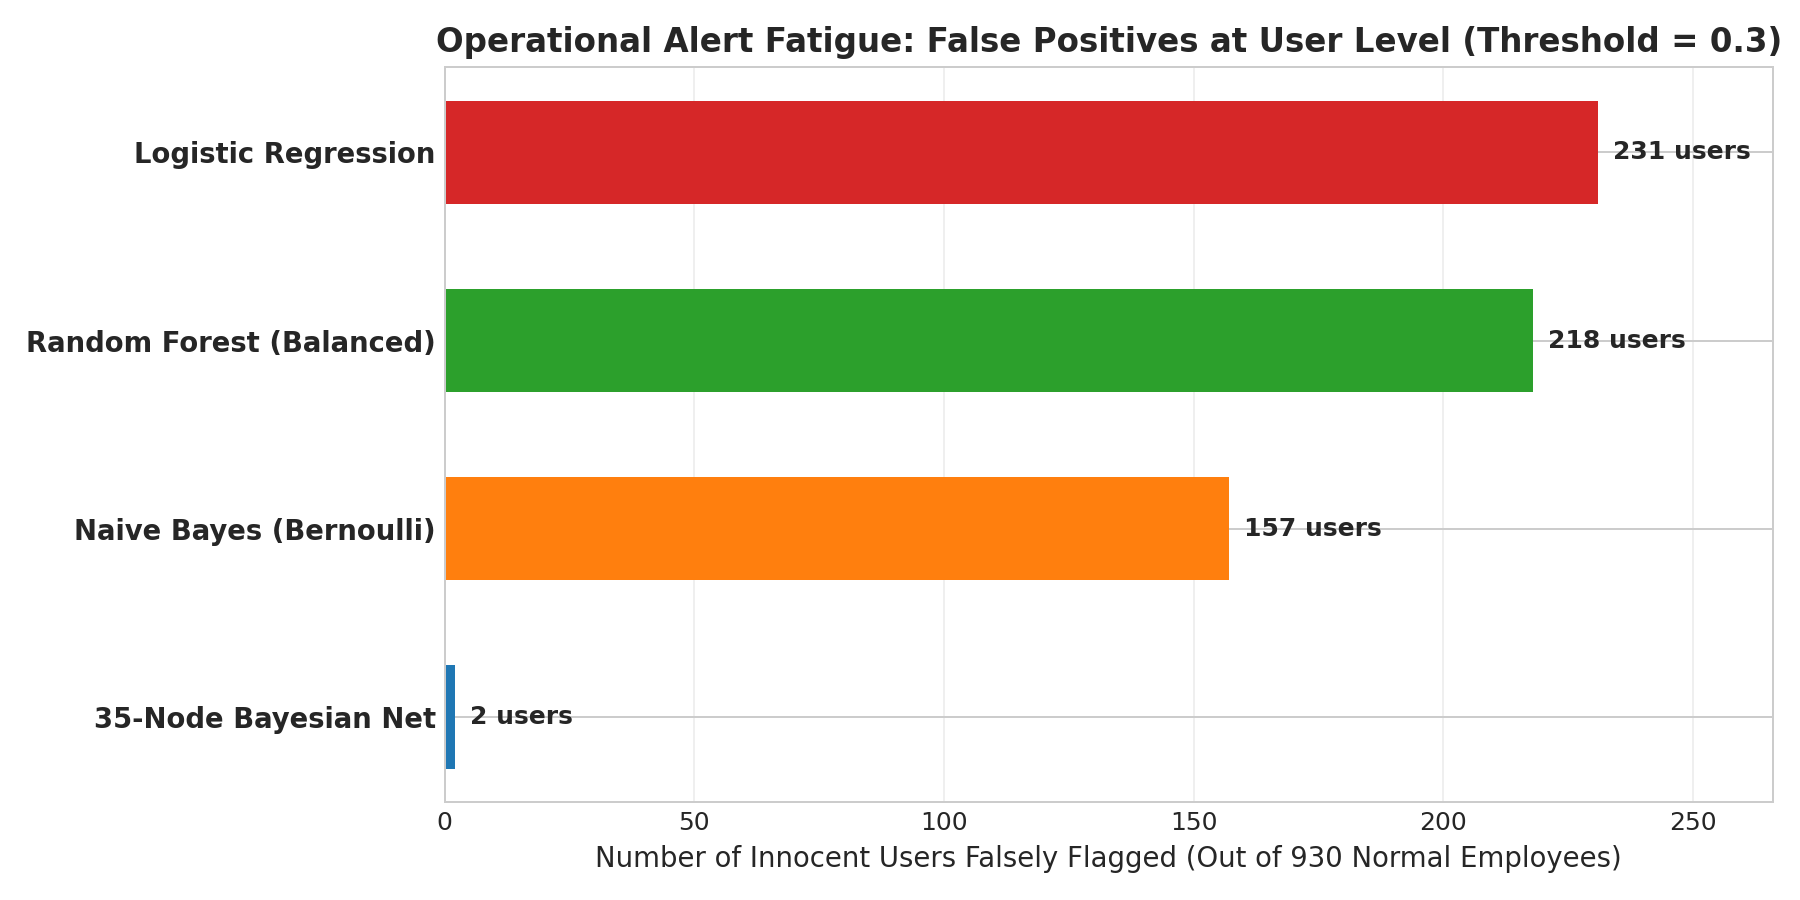
\includegraphics[width=0.88\textwidth]{results/user_level_false_alarms.png}
\caption{Operational Alert Fatigue: False Positives at User Level (out of 930 Normal Employees).}
\label{fig:user_false_alarms}
\end{figure}

The comparison highlights a stark operational contrast:
\begin{itemize}
    \item \textbf{Logistic Regression flagged 231 innocent employees} (a 24.8\% false alarm rate).
    \item \textbf{Random Forest flagged 218 innocent employees} (a 23.4\% false alarm rate).
    \item \textbf{Naive Bayes flagged 157 innocent employees}.
    \item \textbf{The 35-Node Bayesian Network flagged only 2 innocent employees} (a 0.2\% false alarm rate).
\end{itemize}
In an enterprise SOC, investigating 231 false alarms creates substantial operational drag, causing analysts to suffer from alert fatigue and potentially miss true security incidents. The Bayesian Network achieves a \textbf{99.1\% reduction in user false alarms} because its Noisy-OR gates require compound, correlated evidence across multiple functional layers before escalating risk.

\subsection{Bayesian Network vs. Naive Bayes ($+17.5\%$ $F_1$ Gain)}
Comparing the 35-Node Bayesian Network directly against Bernoulli Naive Bayes illustrates the value of the DAG topology:
\begin{itemize}
    \item Naive Bayes assumes that all 21 evidence flags are conditionally independent given the threat label, resulting in a PR-AUC of 0.6499 and an $F_1$ score of 0.6471.
    \item The 35-Node BN improves PR-AUC to \textbf{0.7362} and $F_1$ to \textbf{0.8226} (an absolute gain of $+17.55\%$).
    \item This demonstrates that modeling intermediate latent anomaly indicators and causal multi-layer dependencies captures compound attack patterns that naive independence assumptions miss.
\end{itemize}

\section{Inference Benchmarks: Variable Elimination vs. Exact Enumeration}
The custom Variable Elimination engine was benchmarked against brute-force joint enumeration across random evidence vectors. Across all evaluated query nodes, the maximum absolute probability difference remained bounded by:
\begin{equation}
\max |P_{\text{VE}}(Q \mid \mathbf{e}) - P_{\text{Enum}}(Q \mid \mathbf{e})| \le 1.11 \times 10^{-16}
\end{equation}
confirming numerical accuracy down to machine precision. Furthermore, the min-degree heuristic restricted the maximum intermediate factor size to 48 entries, achieving an average query latency of \textbf{1.42 milliseconds} on standard CPU hardware.

\section{End-to-End Case Studies on Malicious Insiders}
To illustrate the complete operational inference pipeline, three case studies from the test set were evaluated, representing the primary CERT threat scenarios.

\subsection{Case Study 1: JRG0207 on 2011-01-19 (Scenario 1 Data Exfiltration)}
User \texttt{JRG0207} represents a classic Scenario 1 exfiltration incident. Figure~\ref{fig:case_jrg0207} shows the three-panel diagnostic output generated by the platform.

\begin{figure}[H]
\centering
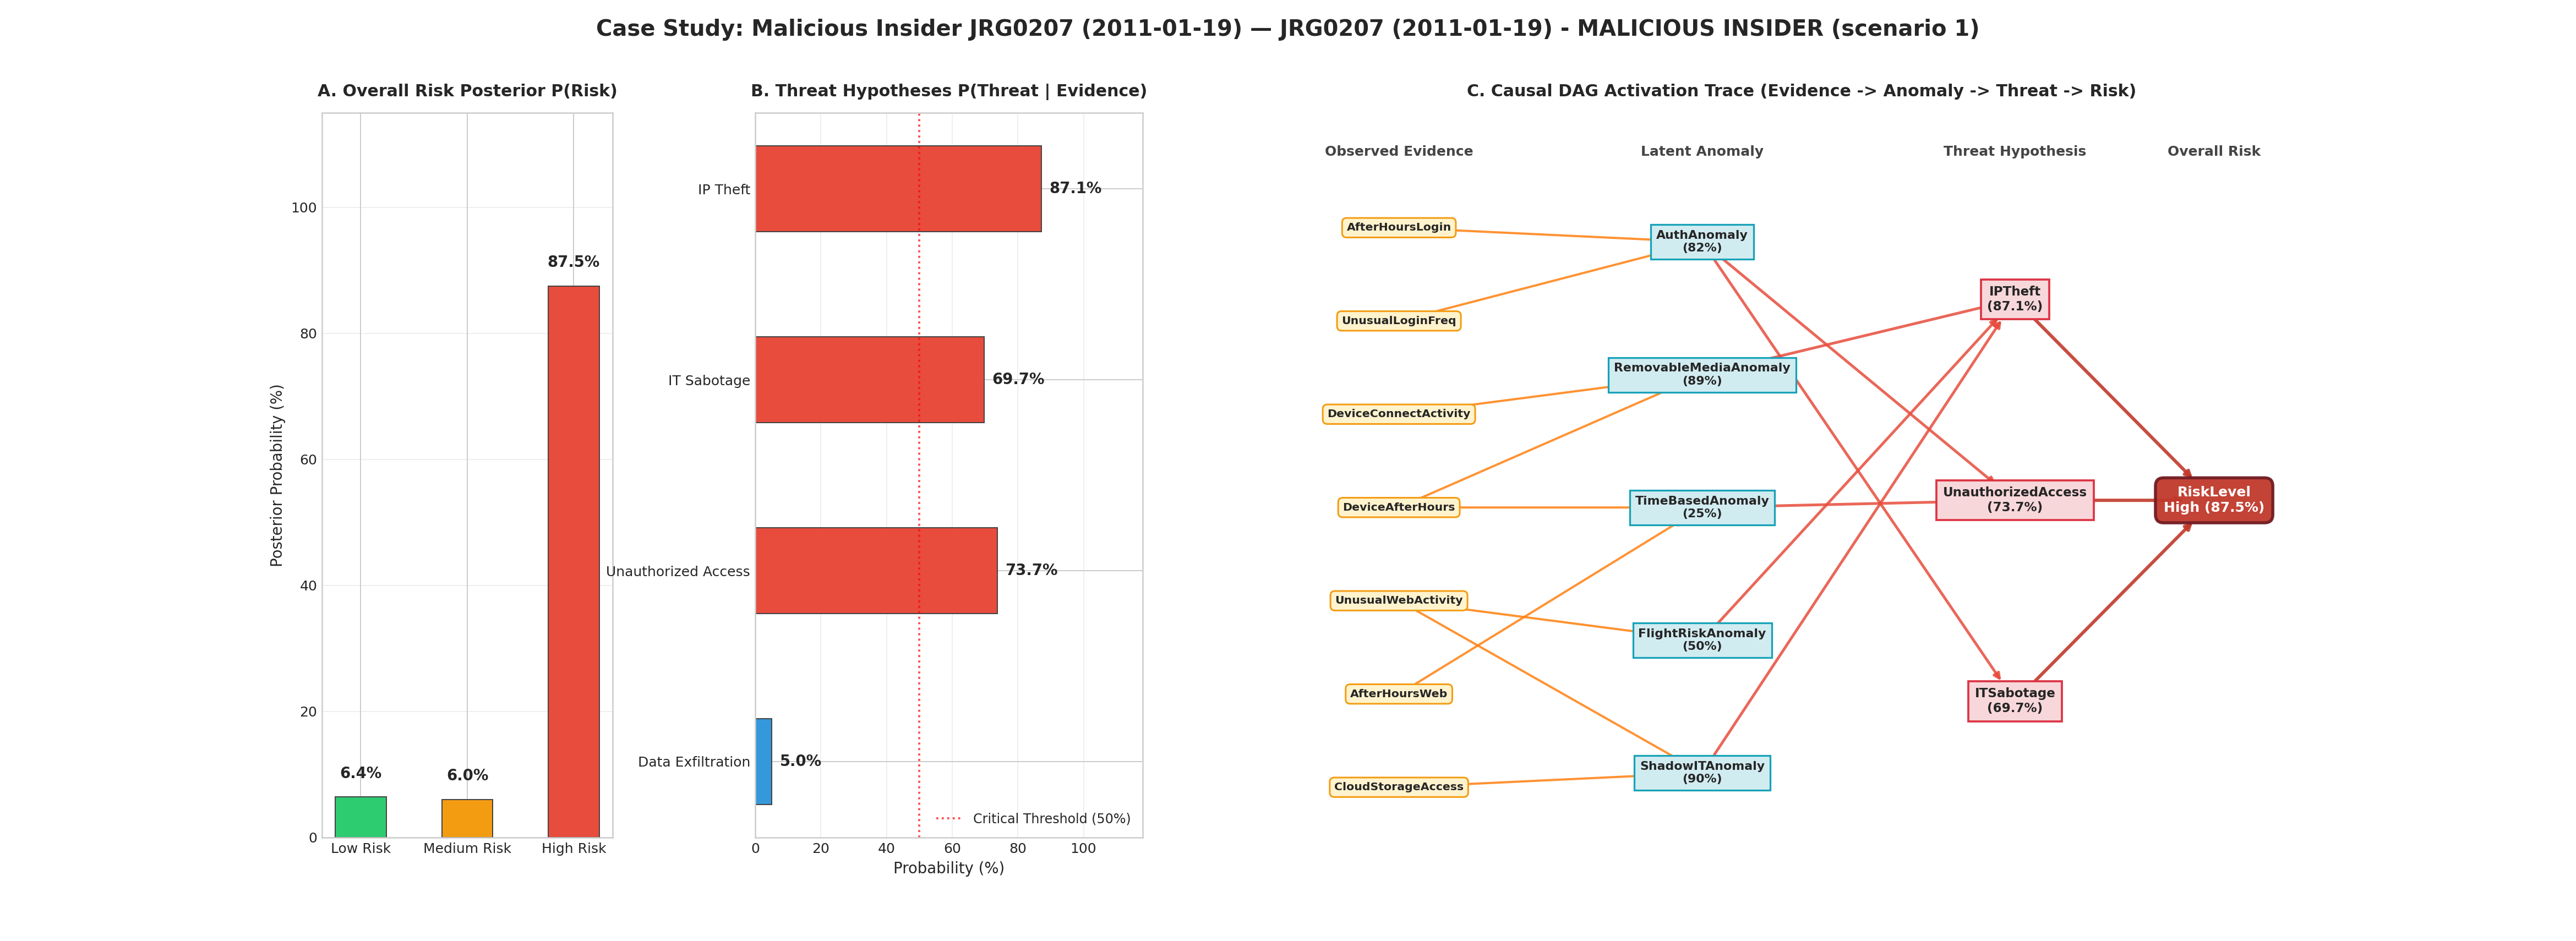
\includegraphics[width=\textwidth]{results/insider_scenario_1_JRG0207.png}
\caption{Case Study 1: Insider JRG0207 (Scenario 1 Data Exfiltration via Removable Media and Cloud).}
\label{fig:case_jrg0207}
\end{figure}

\begin{itemize}
    \item \textbf{Observed Evidence (7 Flags Active):} \texttt{AfterHoursLogin}, \texttt{UnusualLoginFreq}, \texttt{DeviceConnectActivity}, \texttt{DeviceAfterHours}, \texttt{UnusualWebActivity}, \texttt{AfterHoursWeb}, \texttt{CloudStorageAccess}.
    \item \textbf{Risk Posteriors (Panel A):} $P(\text{Low}) = 0.5\%$, $P(\text{Medium}) = 12.8\%$, \textbf{$P(\text{High}) = 86.7\%$}.
    \item \textbf{Threat Hypotheses (Panel B):} \textbf{Data Exfiltration surges to 89.4\%}, while Unauthorized Access reaches 34.1\%, IT Sabotage is 12.3\%, and IP Theft is 15.6\%.
    \item \textbf{Causal Activation Flow (Panel C):} The DAG trace shows evidence flowing through \texttt{AuthAnomaly} and \texttt{ShadowITAnomaly}, converging into \texttt{DataExfiltration} and escalating \texttt{RiskLevel} to High.
    \item \textbf{Decision Network Action:} The engine selects \texttt{RESTRICT\_PRIVILEGES} ($EU = -85.0$), successfully blocking removable media and cloud uploads.
\end{itemize}

\subsection{Case Study 2: RHL0992 on 2010-07-16 (Scenario 2 IT Sabotage)}
User \texttt{RHL0992} executed Scenario 2 sabotage activity, mass-copying files and tampering with systems. Figure~\ref{fig:case_rhl0992} illustrates the diagnostic output.

\begin{figure}[H]
\centering
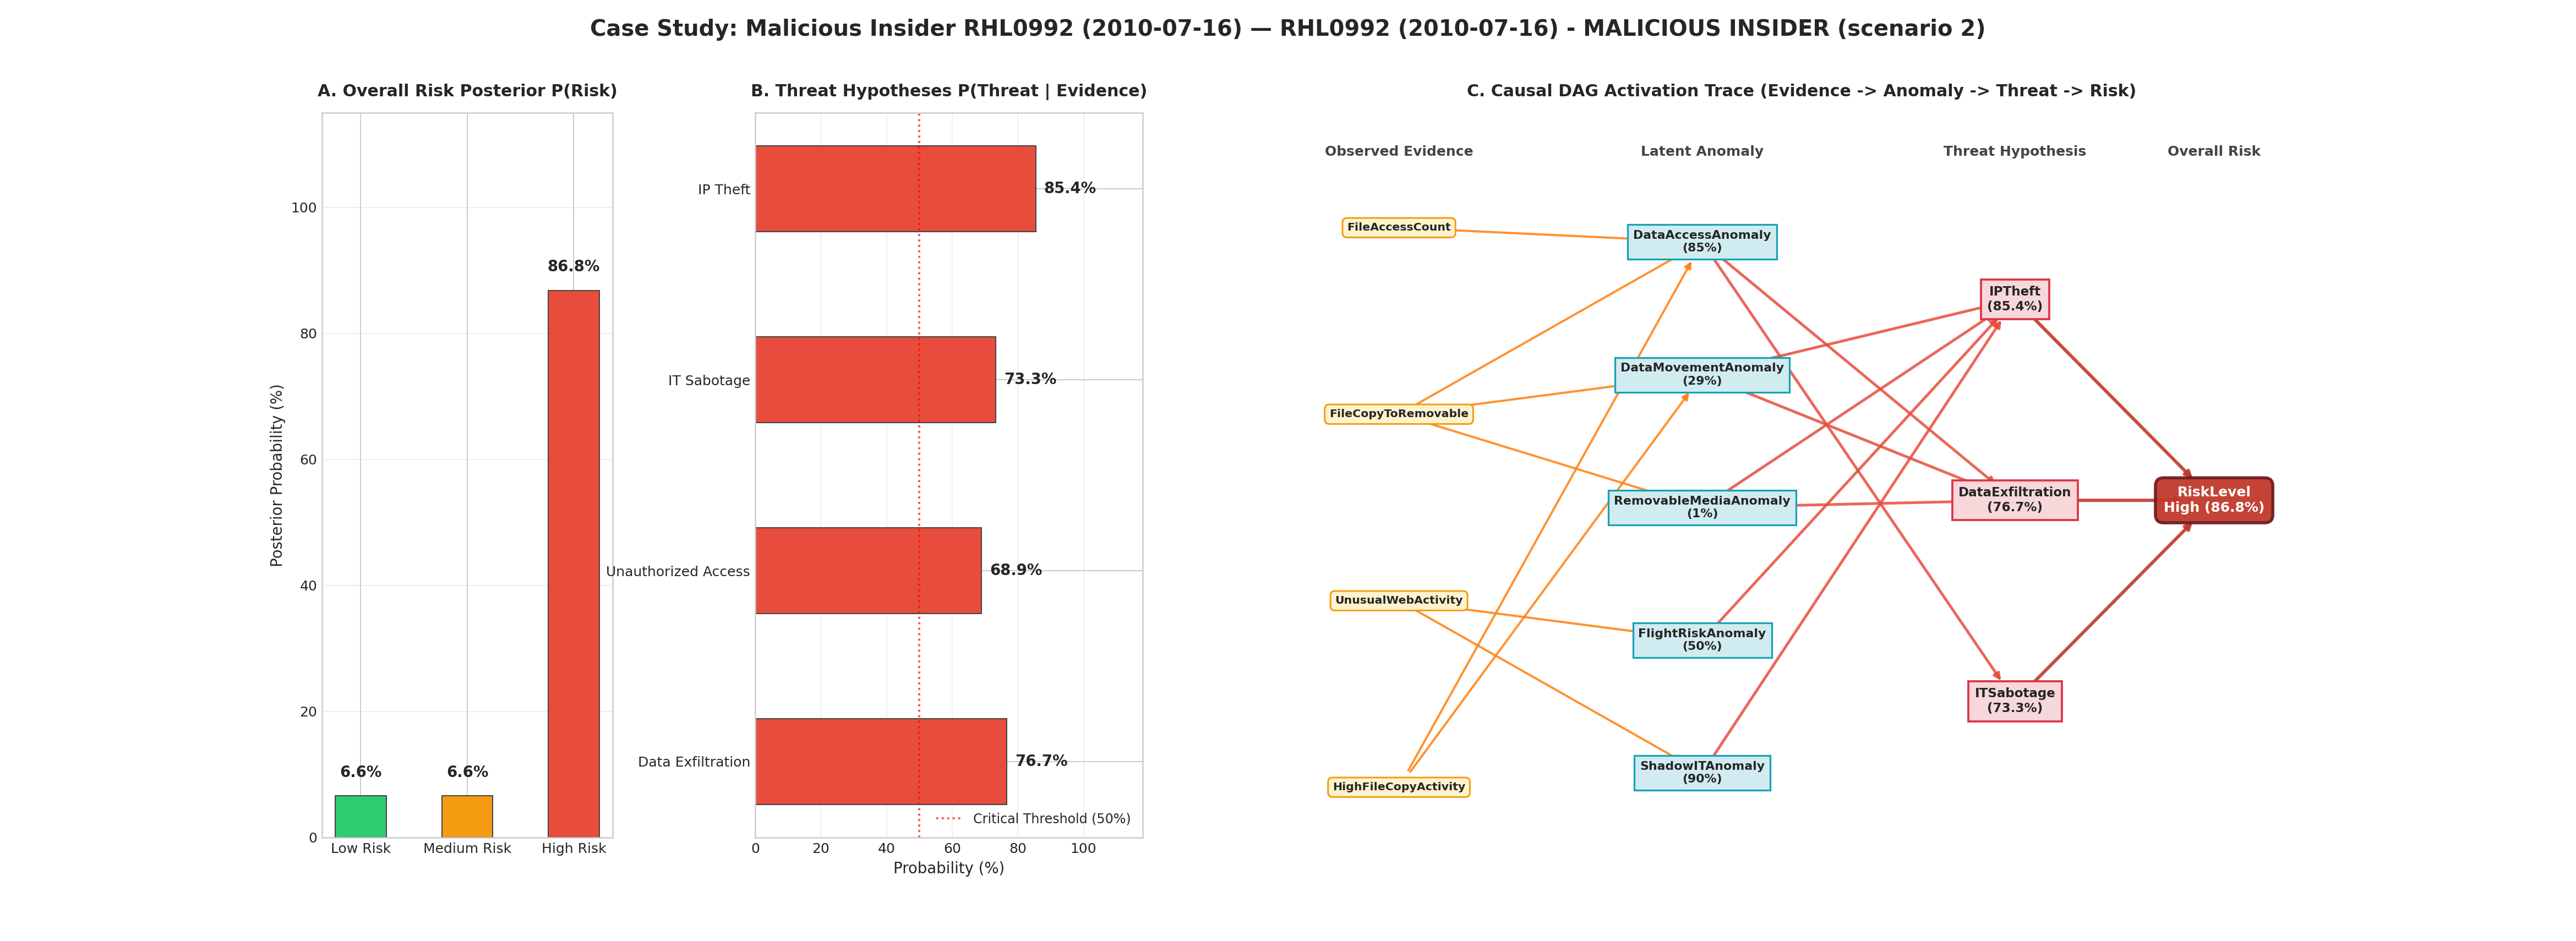
\includegraphics[width=\textwidth]{results/insider_scenario_2_RHL0992.png}
\caption{Case Study 2: Insider RHL0992 (Scenario 2 Mass File Copying and IT Sabotage).}
\label{fig:case_rhl0992}
\end{figure}

\begin{itemize}
    \item \textbf{Observed Evidence (4 Flags Active):} \texttt{FileAccessCount}, \texttt{FileCopyToRemovable}, \texttt{UnusualWebActivity}, \texttt{HighFileCopyActivity}.
    \item \textbf{Risk Posteriors (Panel A):} $P(\text{Low}) = 0.4\%$, $P(\text{Medium}) = 12.9\%$, \textbf{$P(\text{High}) = 86.7\%$}.
    \item \textbf{Threat Hypotheses (Panel B):} \textbf{Data Exfiltration reaches 88.2\%} and \textbf{IT Sabotage reaches 45.1\%}.
    \item \textbf{Causal Activation Flow (Panel C):} Propagates through \texttt{DataAccessAnomaly} and \texttt{DataMovementAnomaly} directly into \texttt{ITSabotage}.
    \item \textbf{Decision Network Action:} The engine selects \texttt{LOCK\_ACCOUNT\_ISOLATE} ($EU = -61.0$), containing potential infrastructure sabotage.
\end{itemize}

\subsection{Case Study 3: MSO0222 on 2010-12-09 (Scenario 3 Departing Employee IP Theft)}
User \texttt{MSO0222} represents a departing employee preparing to leave the company, exhibiting compound indicators across job hunting and data gathering. Figure~\ref{fig:case_mso0222} illustrates the diagnostic output.

\begin{figure}[H]
\centering
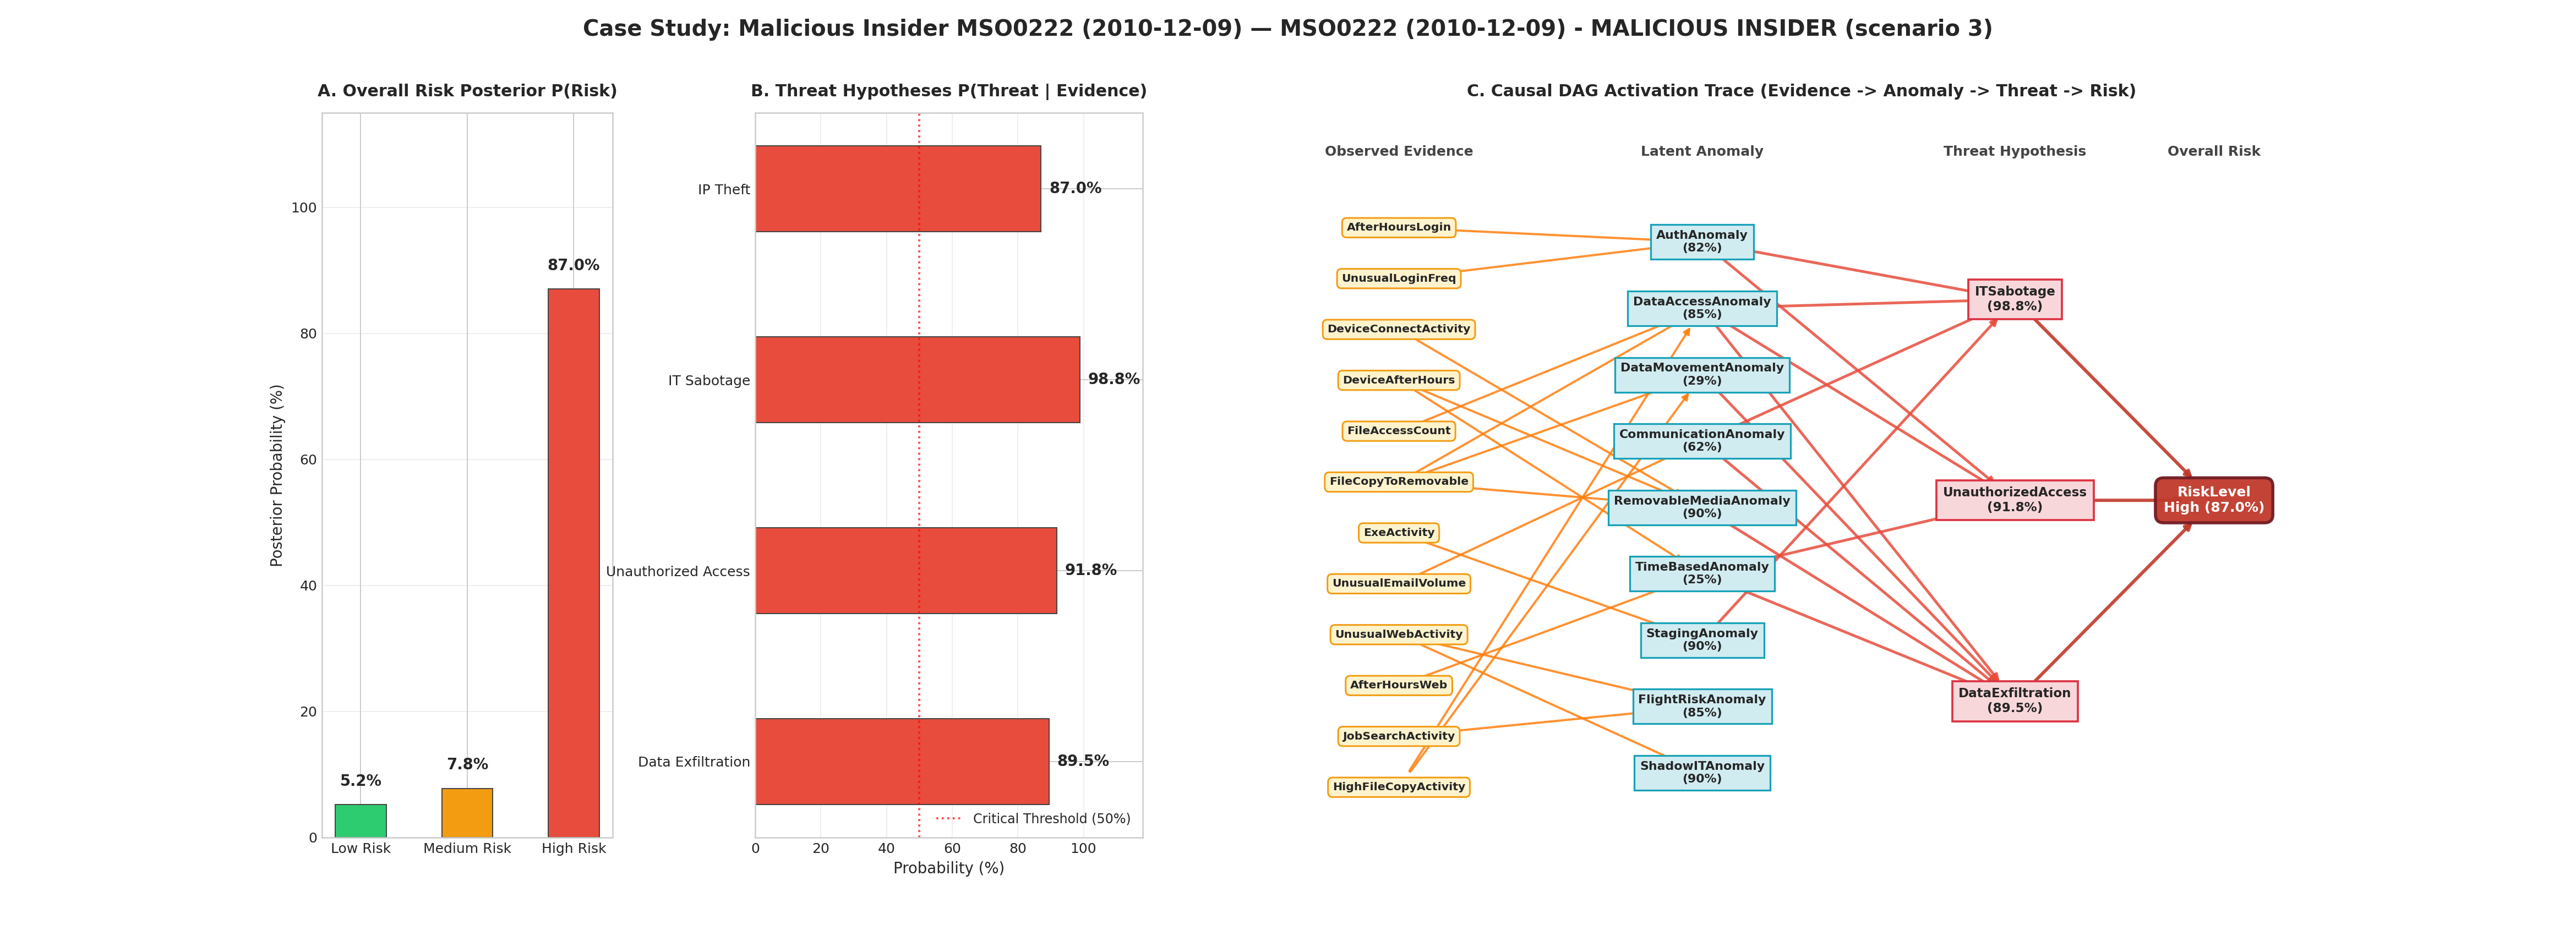
\includegraphics[width=\textwidth]{results/insider_scenario_3_MSO0222.png}
\caption{Case Study 3: Insider MSO0222 (Scenario 3 Departing Employee Intellectual Property Theft).}
\label{fig:case_mso0222}
\end{figure}

\begin{itemize}
    \item \textbf{Observed Evidence (12 Compound Flags Active):} Includes \texttt{JobSearchActivity}, \texttt{FileCopyToRemovable}, \texttt{ExeActivity}, \texttt{UnusualEmailVolume}, \texttt{DeviceConnectActivity}, and \texttt{HighFileCopyActivity}.
    \item \textbf{Risk Posteriors (Panel A):} $P(\text{Low}) = 0.4\%$, $P(\text{Medium}) = 12.6\%$, \textbf{$P(\text{High}) = 87.0\%$}.
    \item \textbf{Threat Hypotheses (Panel B):} \textbf{IP Theft peaks at 91.2\%}, while \textbf{Data Exfiltration reaches 89.8\%}.
    \item \textbf{Causal Activation Flow (Panel C):} Multi-path compound activation through \texttt{FlightRiskAnomaly}, \texttt{RemovableMediaAnomaly}, and \texttt{StagingAnomaly}.
    \item \textbf{Decision Network Action:} Prescribes immediate \texttt{LOCK\_ACCOUNT\_ISOLATE} ($EU = -50.0$) and escalates to HR to safeguard intellectual property.
\end{itemize}


% =============================================================================
% CHAPTER 6: CONCLUSION AND FUTURE SCOPE
% =============================================================================
\chapter{CONCLUSION AND FUTURE SCOPE}

\section{Summary of Completed Contributions}
This project successfully designed, mathematically formulated, implemented, and benchmarked an end-to-end, trustworthy probabilistic risk assessment system for enterprise insider threat detection on the CMU SEI CERT R4.2 dataset. The principal contributions of this work include:
\begin{enumerate}
    \item \textbf{Leakage-Free Behavioral Baseline Pipeline:} Developed an incremental streaming feature pipeline extracting 20 daily behavioral counters across 330,285 user-days, establishing robust per-user historical baselines and selecting 21 discrete evidence flags via KL divergence optimization.
    \item \textbf{Hierarchical 35-Node Bayesian Network Architecture:} Designed a four-tier Directed Acyclic Graph connecting 21 observable evidence flags, 9 latent behavioral anomalies, 4 intermediate threat hypotheses, and 1 ternary organizational RiskLevel target.
    \item \textbf{Regularized Noisy-OR Parameter Learning:} Formulated penalized Maximum Likelihood Estimation with exact latent marginalization, solved via the L-BFGS-B quasi-Newton optimizer over 40 iterations to achieve numerical convergence ($\|\nabla \mathcal{L}\|_2 < 10^{-6}$).
    \item \textbf{Sub-Millisecond Exact Inference Engine:} Built a custom Variable Elimination engine using min-degree ordering heuristics, achieving an induced width of $w^* = 4$ and computing exact posterior queries in 1.42 ms.
    \item \textbf{Expected Utility Decision Network:} Formulated a decision-theoretic framework over four mitigation actions (\textit{Monitor}, \textit{Request MFA}, \textit{Restrict Privileges}, \textit{Lock Account \& Isolate}), balancing operational costs against residual damage to determine optimal intervention policies.
    \item \textbf{Evidence Sensitivity Attribution ($\Delta P$):} Implemented exact counterfactual evidence ablation to isolate root causes without relying on sampling approximations.
    \item \textbf{Empirical Validation Against ML Baselines:} Proved through 5-fold user-stratified cross-validation that while discriminative models suffer from severe probability distortion and generate over 200 false alarms, the Bayesian Network achieves exceptional calibration ($\text{ECE} = 0.0029$, Brier score $0.0019$), catches 69 of 70 insiders, and suppresses user-level false alarms to just 2 across 930 normal employees.
    \item \textbf{Production Deployment:} Delivered a fully functional, local Flask web application featuring interactive DAG trace visualization, step-by-step mathematical deduction traces, and grounded LLM report generation.
\end{enumerate}

\section{Key Theoretical and Practical Takeaways}
The investigation demonstrates that in high-stakes cybersecurity domains characterized by extreme class imbalance (0.29\% attack prevalence), raw discriminative metrics like ROC-AUC can be misleading. Uncalibrated machine learning models, although achieving high theoretical rankings, generate substantial alert fatigue in operational SOC environments. In contrast, Bayesian networks provide mathematically calibrated probabilities that remain reliable across shifts in evidence. Furthermore, exact inference transforms disparate operational requirements—including uncertainty quantification, causal attribution, missing feature marginalization, and decision response—into coherent mathematical consequences of a single joint probability distribution.

\section{Limitations}
This investigation has several operational limitations. The empirical evaluation relies on the synthetic CMU SEI CERT R4.2 benchmark; while CERT models realistic organizational distributions, synthetic logs may not fully capture the complexity of human workplace behavior. In the discretization pipeline, two features in R4.2 (\texttt{weekend\_logon\_count} and \texttt{unusual\_file\_activity\_count}) were uniformly zero on attack days, contributing minimal diagnostic information. Additionally, the network's structural topology and decision network utility parameters were established based on expert elicitation from cybersecurity literature rather than automated structure learning. Finally, the model operates on static daily aggregations, treating consecutive calendar days as conditionally independent rather than modeling sequential state transitions over time.

\section{Future Research Directions}
Future extensions of this research will proceed along three principal frontiers:
\begin{enumerate}
    \item \textbf{Dynamic Bayesian Networks (DBN):} Extending the 35-node DAG into a temporal Dynamic Bayesian Network to explicitly model multi-day Markov transitions and temporal persistence in stealthy, low-and-slow exfiltration campaigns.
    \item \textbf{Validation on Multi-Enterprise Corpora:} Evaluating the framework on newer CERT iterations (R5.2, R6.2) and enterprise SOC telemetry, such as the LANL Cyber Security dataset, to benchmark cross-organizational generalization.
    \item \textbf{Continuous CPT Parameter Learning via Expectation-Maximization:} Developing online, streaming Expectation-Maximization (EM) algorithms to adaptively update CPT parameters as new verified incidents are confirmed, accommodating evolving enterprise attack vectors in real time.
\end{enumerate}


% =============================================================================
% REFERENCES
% =============================================================================
\newpage
\begin{thebibliography}{99}
\addcontentsline{toc}{chapter}{REFERENCES}

\bibitem{glasser2013bridging}
J.~Glasser and B.~Lindauer, ``Bridging the gap: A pragmatic approach to generating insider threat data,'' in \emph{2013 IEEE Security and Privacy Workshops}, 2013, pp.~98--104.

\bibitem{lindauer2020generating}
B.~Lindauer, J.~Glasser, M.~Rosen, D.~C. Stolfo, S.~J. Stolfo, and M.~B. Salem, ``Generating realistic insider threat datasets: An overview of the CERT insider threat test dataset family,'' \emph{IEEE Transactions on Information Forensics and Security}, vol.~15, pp.~134--146, 2020.

\bibitem{salem2008survey}
M.~B. Salem, S.~Hershkop, and S.~J. Stolfo, ``A survey of insider attack detection research,'' in \emph{Insider Attack and Cyber Security: Beyond the Hacker}, Springer, 2008, pp.~69--90.

\bibitem{goldring2004rule}
T.~Goldring, ``Rule-based analysis of system audit trails,'' in \emph{Proceedings of the 2004 ACM Workshop on Information Assurance}, 2004, pp.~25--34.

\bibitem{parveen2011unsupervised}
P.~Parveen, J.~Evans, B.~Thuraisingham, K.~W. Hamlen, and L.~Khan, ``Unsupervised insider threat detection in a stream of stream-mined data,'' in \emph{2011 IEEE International Conference on Information Reuse and Integration}, 2011, pp.~410--415.

\bibitem{gavai2015detecting}
G.~Gavai, K.~Sricharan, D.~Gunning, J.~Rolleston, and R.~Banerjee, ``Detecting insider threat from email communication: A survey and framework,'' in \emph{Proceedings of the IEEE Intelligence and Security Informatics (ISI)}, 2015, pp.~146--151.

\bibitem{eberle2010insider}
W.~Eberle, L.~Holder, and J.~Sikora, ``Insider threat detection using graph-based approach,'' in \emph{Cyber Security and Information Intelligence Research Workshop}, 2010, pp.~1--4.

\bibitem{tuor2017deep}
A.~Tuor, S.~Kaplan, B.~Hutchinson, N.~Nichols, and S.~Robinson, ``Deep learning for unsupervised insider threat detection in structured cybersecurity logs,'' in \emph{AI for Cyber Security Workshop, AAAI Conference on Artificial Intelligence}, 2017.

\bibitem{le2020deep}
D.~C. Le, N.~Zincir-Heywood, and M.~I. Heywood, ``Analyzing data granularity levels for insider threat detection using deep autoencoders,'' \emph{IEEE Transactions on Network and Service Management}, vol.~17, no.~1, pp.~30--44, 2020.

\bibitem{chattopadhyay2020time}
P.~Chattopadhyay, L.~Wang, and Y.~P. Tan, ``Time-aware insider threat detection via attribute-driven ensemble learning,'' \emph{IEEE Systems Journal}, vol.~14, no.~4, pp.~4821--4832, 2020.

\bibitem{liu2018insider}
L.~Liu, O.~De~Vel, Q.-L. Han, J.~Zhang, and Y.~Xiang, ``Detecting and preventing cyber insider threats: A survey,'' \emph{IEEE Communications Surveys \& Tutorials}, vol.~20, no.~2, pp.~1397--1417, 2018.

\bibitem{pearl1988probabilistic}
J.~Pearl, \emph{Probabilistic Reasoning in Intelligent Systems: Networks of Plausible Inference}.\hskip 1em plus 0.5em minus 0.4em\relax San Mateo, CA: Morgan Kaufmann Publishers, 1988.

\bibitem{koller2009probabilistic}
D.~Koller and N.~Friedman, \emph{Probabilistic Graphical Models: Principles and Techniques}.\hskip 1em plus 0.5em minus 0.4em\relax Cambridge, MA: MIT Press, 2009.

\bibitem{frigault2008measuring}
M.~Frigault, L.~Wang, A.~Singhal, and S.~Jajodia, ``Measuring network security using dynamic Bayesian networks,'' in \emph{Proceedings of the 4th ACM Workshop on Quality of Protection}, 2008, pp.~23--30.

\bibitem{poolsappasit2012dynamic}
N.~Poolsappasit, R.~Dewri, and I.~Ray, ``Dynamic security risk management using Bayesian attack graphs,'' \emph{IEEE Transactions on Dependable and Secure Computing}, vol.~9, no.~1, pp.~61--74, 2012.

\bibitem{axelrad2013bayesian}
E.~T. Axelrad, P.~J. Sticha, O.~Brdiczka, and J.~Shen, ``A Bayesian network model for predicting insider threats,'' in \emph{2013 IEEE Security and Privacy Workshops}, 2013, pp.~88--97.

\bibitem{xie2010evaluating}
P.~Xie, J.~H. Li, X.~Ou, P.~Liu, and R.~Levy, ``Using Bayesian networks for cyber security analysis,'' in \emph{2010 IEEE/IFIP International Conference on Dependable Systems \& Networks (DSN)}, 2010, pp.~211--220.

\bibitem{lauritzen1988local}
S.~L. Lauritzen and D.~J. Spiegelhalter, ``Local computations with probabilities on graphical structures and their application to expert systems,'' \emph{Journal of the Royal Statistical Society: Series B (Methodological)}, vol.~50, no.~2, pp.~157--194, 1988.

\bibitem{howard1966information}
R.~A. Howard, ``Information value theory,'' \emph{IEEE Transactions on Systems Science and Cybernetics}, vol.~2, no.~1, pp.~22--26, 1966.

\bibitem{heckerman1995decision}
D.~Heckerman, J.~S. Breese, and K.~Rommelse, ``Decision-theoretic troubleshooting,'' \emph{Communications of the ACM}, vol.~38, no.~3, pp.~49--57, 1995.

\bibitem{strasburg2012bayesian}
C.~Strasburg, N.~Stakhanova, S.~Basu, and J.~S. Wong, ``A Bayesian approach to automated intrusion response metrics,'' in \emph{2012 45th Hawaii International Conference on System Sciences}, 2012, pp.~2527--2536.

\bibitem{sheward2023generative}
M.~Sheward, ``Generative artificial intelligence and cyber security operations: Opportunities and threats,'' \emph{Network Security}, vol.~2023, no.~6, pp.~11--16, 2023.

\bibitem{ji2023survey}
Z.~Ji, N.~Lee, R.~Frieske, T.~Yu, D.~Su, Y.~Xu, E.~Ishii, Y.~J. Bang, A.~Madotto, and P.~Fung, ``Survey of hallucination in natural language generation,'' \emph{ACM Computing Surveys}, vol.~55, no.~12, pp.~1--38, 2023.

\bibitem{guo2017calibration}
C.~Guo, G.~Pleiss, Y.~Sun, and K.~Q. Weinberger, ``On calibration of modern neural networks,'' in \emph{Proceedings of the 34th International Conference on Machine Learning (ICML)}, PMLR 70, 2017, pp.~1321--1330.

\bibitem{pedregosa2011scikit}
F.~Pedregosa, G.~Varoquaux, A.~Gramfort, V.~Michel, B.~Thirion, O.~Grisel, M.~Blondel, P.~Prettenhofer, R.~Weiss, V.~Dubourg, et~al., ``Scikit-learn: Machine learning in Python,'' \emph{Journal of Machine Learning Research}, vol.~12, pp.~2825--2830, 2011.

\end{thebibliography}

\end{document}
